\subsection{Objetivos}

El desarrollo de una PCB se considera una de las partes esenciales de este proyecto y por lo tanto su importancia es máxima.

El objetivo principal que persigue el diseñar y construir una PCB en este proyecto es el de dotar al sistema de un centro de cómputo principal, el cual es utilizado para procesar las \textbf{ordenes} de S1, realizar los cálculos pertinentes y ejecutar las acciones necesarias sobre la estructura del brazo robótico. La PCB por lo tanto, se encarga de alojar el microcontrolador dsPIC, así como todos los periféricos necesarios para establecer la comunicación con S1, realizar el control de los actuadores y monitorizar el estado del manipulador.

\subsection{Componentes principales}

En general, se podría decir que los componentes de la PCB se clasifican en tres categorías principales:
\begin{itemize}
    \item Componentes de alimentación eléctrica.
    \item Microcontrolador y componentes auxiliares para su correcto funcionamiento.
    \item Periféricos destinados a control de actuadores y canales de comunicación.
\end{itemize}

En primer lugar, los componentes de alimentación eléctrica son aquellos que forman el circuito de alimentación del microcontrolador así como de los actuadores. El circuito eléctrico de alimentación de la PCB se ha diseñado para poder alimentar de forma simultánea al microcontrolador y a cada uno de los cuatro servomotores y, por lo tanto, está formado por dos etapas:
\begin{itemize}
    \item La PCB recibe una tensión de entrada de $9V$ y una corriente de entre $1.8A - 2A$ mediante una clema. Posteriormente, esta tensión de alimentación será reducida y adaptada para alimentar a cada una de las etapas de la PCB, es decir, al microcontrolador y servomotores.
    \item En la primera etapa se reduce el voltaje de alimentación principal a $6V$ y $0.4A$ aproximadamente para cada uno de los servomotores, utilizando para ello un regulador LM317 para cada servomotor. Esta alimentación se realiza mediante clemas, a las cuales se deben conectar la alimentación de los motores.
    
    \item En la segunda etapa se reduce el voltaje de alimentación principal a $3.3V$ y $0.15A$ aproximadamente con el objetivo de alimentar el microcontrolador, utilizando para ello reguladores LM317 y A1117H. Esta alimentación se realiza mediante pistas únicamente.
\end{itemize}

En segundo lugar, el microcontrolador y sus componentes auxiliares representan el núcleo de la PCB:
\begin{itemize}
    \item El dsPIC se encuentra localizado en el centro de la PCB y de él surgen todas las conexiones necesarias hacia los periféricos.
    \item Los componentes auxiliares del microcontrolador son componentes eléctricos que aseguran el correcto funcionamiento del dsPIC, así como su seguridad. En el caso específico de este microcontrolador, es necesario incluir varios condensadores en sus pines de alimentación.
\end{itemize}

En último lugar, se han utilizado los siguientes periféricos:

\begin{itemize}
    \item Cristal de cuarzo: mediante este componente, se genera una señal de reloj precisa y de buena calidad. Su frecuencia es de $7MHz$ y \textbf{sera} recibida por el microcontrolador para ser usada como la señal de reloj principal del sistema.
    
    \item Puerto de programación: mediante este periférico se puede conectar la sonda de programación del microcontrolador y por lo tanto es un elemento con especial importancia y relevancia dentro del sistema.
    
    \item Puerto TRIS: mediante este periférico se pueden recibir señales digitales y analógicas, las cuales son procesadas por el microcontrolador. En este proyecto, estos puertos se utilizan para monitorizar los finales de carrera de la estructura del brazo robótico.
    \item Puerto PWM: mediante este periférico se pueden generar señales PWM, es decir, señales digitales cuadradas y con un ancho de pulso variable, las cuales son completamente necesarias para controlar los servomotores.
    
    \item UART: mediante este periférico se establece un canal de comunicación \textit{hardware} con S1, el cual se usa para recibir órdenes, movimientos y realimentar su resultado de vuelta a S1.
    
    \item LEDs de estado: mediante este periférico se muestra el estado del sistema usando tres diodos LED.
\end{itemize}

Mediante esta descripción general de la PCB y sus componentes se pretende brindar una idea global de la misma, así como de cual es su papel dentro del proyecto. En los apartados siguientes se describe en términos técnicos los elementos de esta PCB, así como el proceso de diseño y fabricación llevado a cabo.

\subsection{Diseño lógico y diagrama esquemático}

El primer paso llevado a cabo durante el diseño de la PCB ha sido realizar un diseño lógico de alto nivel, en el cual se muestran las conexiones lógicas que existen entre los componentes; se trata, por lo tanto, del diseño con mayor nivel de abstracción y que tiene como objetivo establecer un diseño de primer nivel, es decir, la primera toma de contacto con el plano de la PCB.

El diseño lógico se lleva a cabo mediante un diagrama esquemático que contiene dos tipos de elementos: huella lógica de cada uno de los componentes y las conexiones entre ellos. Este diagrama se ha llevado a cabo utilizando la herramienta \textit{Schematic Layout Editor} incluida en KiCad.

El diagrama esquemático está dividido en dos partes principales, las cuales facilitan la compresión del mismo:
\begin{itemize}
    \item Diagrama esquemático del circuito de alimentación.
    \item Diagrama esquemático del microcontrolador y sus periféricos.
\end{itemize}

En primer lugar, se procede a describir detalladamente el diagrama esquemático del circuito de alimentación, el cual contiene las dos etapas de alimentación, siendo los principales componentes usados los reguladores de voltaje LM317, L7805CV y AZ1117H.

La clema principal de alimentación recibe $9V$ y $1.8A$ aproximadamente. Esta alimentación debe ser provista externamente mediante una fuente de alimentación regulable o similares. 

Conectados directamente a la clema principal, se encuentran los reguladores de tensión correspondientes a las dos etapas de alimentación:
\begin{itemize}
    \item La primera está formada por cuatro reguladores LM317, los cuales alimentan cada uno de los servomotores. En dicha etapa se reduce el voltaje de $9V$ a $5.5V$.
    
    \item La segunda está formada por un regulador de tensión L7805CV y un AZ1117H. En dicha etapa de alimentación se reduce el voltaje de $9V$ a $5V$ usando el primer regulador, y de $5V$ a $3.3V$ usando el segundo.
\end{itemize}

En particular, el LM317 es un regulador convencional que recibe una tensión que recibe una tensión continua de entrada de entre $3V$ - $40V$, y provee una tensión continua salida de entre $1.25V$ - $37V$. Además, la relación entre la tensión de entrada y salida depende del dimensionado de dos resistencias auxiliares. El conexionado sugerido por el fabricante es el siguiente y se ha obtenido del \textit{datasheet} del regulador:

\begin{figure}[H]
    \centering 
    \includegraphics[width=.6\linewidth]{pictures/LM317 conexionado.PNG}
    \caption{Diagrama de conexionado \textbf{INSERTE CITA AL DATASHEET}}
    \label{fig:CAMBIAR!!!!!!!!!!}
\end{figure}

La ecuación de funcionamiento que ofrece el fabricante para el regulador LM317 es la siguiente:
\begin{equation}
    V_{OUT} = V_{REF} \cdot \left( 1 + \frac{R_2}{R_1}\right) + I_{ADJ} \cdot R_2
\end{equation}

La ecuación anterior debe ser usada para realizar los cálculos pertinentes sobre el valor de las resistencias $R_2$ y $R_1$. Se tienen en cuenta, además, dos observaciones necesarias para la correcta aplicación de la ecuación anterior:
\begin{itemize}
    \item Por definición, el fabricante establece el valor $V_{REF}$ en $1.25V$.
    \item Por motivos de construcción del regulador, la corriente $I_{ADJ}$ tiene un valor máximo de $100 \mu A$ y, por lo tanto, el término de la ecuación que la involucra puede ser despreciado.
\end{itemize}

Se obtiene entonces que la ecuación funcional a utilizar en el cálculo de $R_1$ y $R_2$ es:

\begin{equation}
    V_{OUT} = 1.25 \cdot \left( 1 + \frac{R_2}{240}\right) 
\end{equation}

Teniendo en cuenta los voltajes de alimentación requeridos para las dos etapas de alimentación de la PCB, se han realizado los siguientes cálculos para los valores de la resistencia $R_1$ y $R_2$:
\begin{itemize}
    \item Primera etapa, alimentación de servomotores, $5.5V$ y $0.4A$ requeridos:
    \begin{equation}
        5.5 = 1.25 \cdot \left( 1 + \frac{R_2}{R_1}\right) 
    \end{equation}
    Por disponibilidad de materiales, se ha decidido escoger los valores $150\Omega$ y $500\Omega$ para las resistencias $R_1$ y $R_2$ respectivamente. Tomando en cuenta dichos valores y utilizando la ecuación anterior, se obtiene una reducción de voltaje de $9V$ a $5.41V$, voltaje suficiente para alimentar los servomotores.
\end{itemize}

Aplicando el conexionado recomendado por el fabricante y los cálculos para el valor de las resistencias se obtiene finalmente el diagrama esquemático del circuito de alimentación de los servomotores:

\begin{figure}[H]
    \centering 
    \includegraphics[width=.85\linewidth]{pictures/EsquematicoAlimentaciónServos.PNG}
    \caption{Diagrama esquemático del circuito de alimentación de los servomotores}
    \label{fig:CAMBIAR!!!!!!!!!!}
\end{figure}

El funcionamiento de los reguladores L7805CV y AZ1117H es simple:
\begin{itemize}
    \item El regulador L7805CV recibe un voltaje de entre $7V$ - $35V$ y provee un voltaje de salida fijo de $5V$. Su conexionado se realiza utilizando dos condensadores auxiliares, tal y como se describe en el \textit{datasheet} del componente:
    
    \begin{figure}[H]
    \centering 
    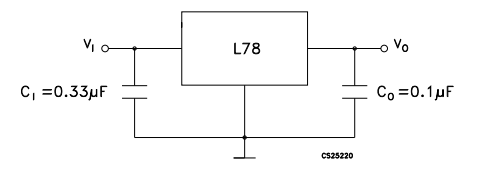
\includegraphics[width=.75\linewidth]{pictures/L7805Datasheet.PNG}
    \caption{Diagrama de conexionado del regulador L7805 \textbf{INSERTE CITA DATASHEET}.}
    \label{fig:CAMBIAR!!!!!!!!!!}
    \end{figure}
    
    \item El regulador AZ1117H recibe un voltaje de hasta $15V$ y provee un voltaje de salida fijo de $3.3V$. Su conexionado se realiza de la misma forma que para el regulador anterior, tal y como se describe en el \textit{datasheet} del componente:
    
    \begin{figure}[H]
    \centering 
    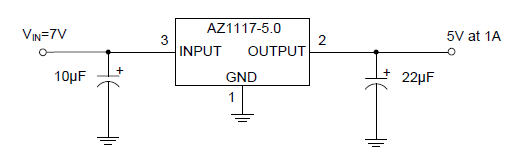
\includegraphics[width=.75\linewidth]{pictures/AZ1117Hdatasheet.PNG}
    \caption{Diagrama de conexionado del regulador AZ1117H \textbf{INSERTE CITA DATASHEET}.}
    \label{fig:CAMBIAR!!!!!!!!!!}
    \end{figure}
    
    En el diagrama anterior se utiliza el modelo que ofrece regulación de voltaje a $5V$. Sin embargo, el modelo usado en el proyecto es el que ofrece regulación de voltaje a $3.3V$, siendo su conexionado exactamente igual.
    
\end{itemize}

Teniendo en cuenta la información expuesta anteriormente, se ha decidido conectar en serie ambos reguladores, consiguiendo de esta forma una regulación de $9V$ a $5V$ y posteriormente una regulación de $5V$ a $3.3V$. El diagrama esquemático final es el siguiente:

    \begin{figure}[H]
    \centering 
    \includegraphics[width=.95\linewidth]{pictures/EsquematicoAlimentaciónPic.PNG}
    \caption{Diagrama esquemático de la etapa de alimentación del microcontrolador.}
    \label{fig:CAMBIAR!!!!!!!!!!}
    \end{figure}

Es importante destacar tres aspectos:
\begin{itemize}
    \item La primera etapa de alimentación incluye clemas para su conexionado con los servomotores.
    \item La segunda etapa de alimentación incluye un puerto de cuatro pines, los cuales se usan para alimentar los micro-interruptores y el microcontrolador.
    \item El conexionado de todos los reguladores se ha realizado en paralelo, dedicando un regulador para cada servomotor así como para el microcontrolador. El objetivo de esta configuración es garantizar una vía de alimentación independiente para cada componente, reduciendo las interferencias de alimentación entre los reguladores y diferenciando la etapa de alimentación de los servomotores y microcontrolador.
\end{itemize}

En segundo lugar se procede a describir detalladamente el diagrama esquemático del microcontrolador y sus periféricos. A continuación se muestra el diagrama esquemático final y posteriormente se detallará cada uno de los periféricos:

\begin{figure}[H]
    \centering 
    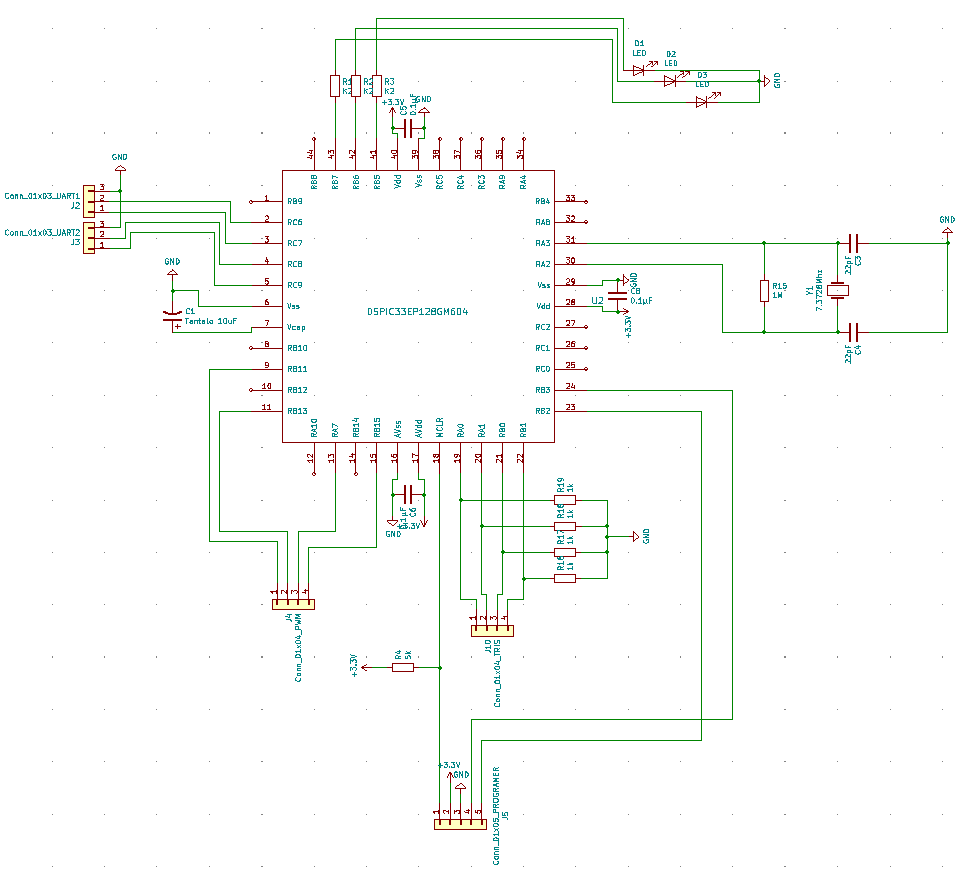
\includegraphics[width=.95\linewidth]{pictures/EsquematicoMicrocontrolador.PNG}
    \caption{Diagrama esquemático del microcontrolador y sus periféricos.}
    \label{fig:CAMBIAR!!!!!!!!!!}
\end{figure}

Primeramente, es importante describir los condensadores auxiliares necesarios para el correcto funcionamiento del microcontrolador, los cuales se encuentran conectados en los pines de alimentación del mismo. Su conexionado es sugerido por el fabricante en el \textit{datasheet} según el siguiente esquema, tratándose así de la configuración mínima recomendada:

\begin{figure}[H]
    \centering 
    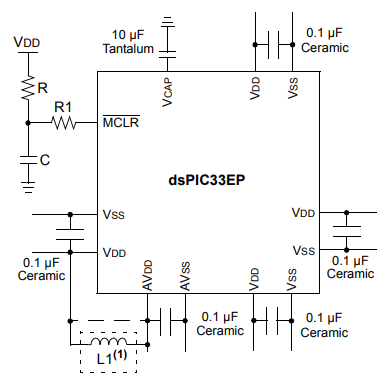
\includegraphics[width=.7\linewidth]{pictures/Minimun.PNG}
    \caption{Conexionado mínimo del microcontrolador.}
    \label{fig:CAMBIAR!!!!!!!!!!}
\end{figure}

Todos los condensadores han sido conectados a los pines descritos por el fabricante y escogidos teniendo en cuenta las características técnicas de los mismos, también descritas en el \textit{datasheet}.

A continuación, se describe el conexionado del resto de puertos y periféricos:

\begin{itemize}
    \item Cristal de cuarzo: en términos técnicos, se trata de un cristal de $7.32MHz$, perfectamente válido para el microcontrolador usado en el proyecto:
    
    \begin{figure}[H]
    \centering 
    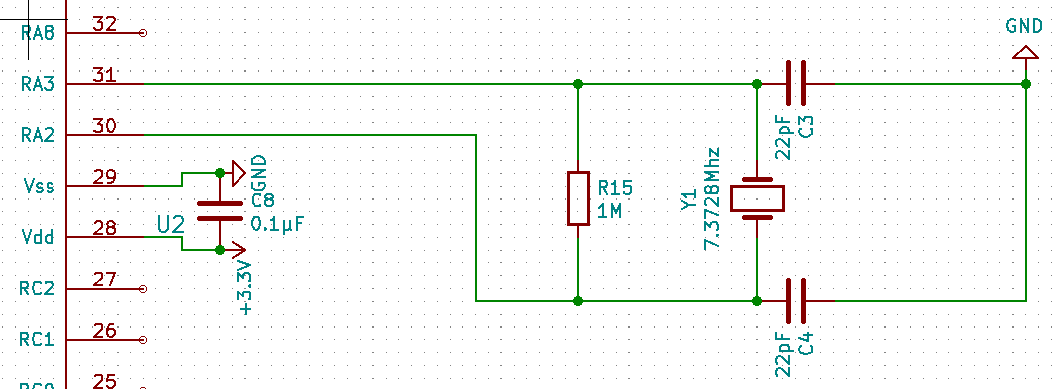
\includegraphics[width=.7\linewidth]{pictures/Cristal.PNG}
    \caption{Diagrama esquemático del conexionado del generador de señales.}
    \label{fig:CAMBIAR!!!!!!!!!!}
    \end{figure}
    
    Su conexionado se realiza con los pines 32 y 31 del microcontrolador, siguiendo la estructura de la imagen anterior, empleando también una resistencia de $1 M \Omega$ y dos condensadores de $22 pF$.
    
    \item Puerto de programación mediante sonda: El conector que recibe la sonda debe tener una estructura específica y se describe en el \textit{datasheet} de la misma:
    
    \begin{figure}[H]
    \centering 
    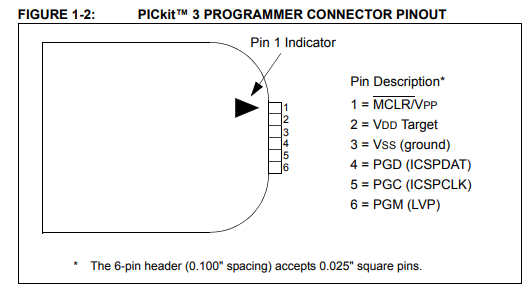
\includegraphics[width=.5\linewidth]{pictures/Sonda.PNG}
    \caption{\textit{Pinout} del conector de la sonda de programación \textbf{INSERTE CITA AQUÍ}.}
    \label{fig:CAMBIAR!!!!!!!!!!}
    \end{figure}
    
     Cabe destacar que el pin 18 o MCLR debe tener un conexionado específico en el que se emplea una resistencia \textit{pull-up}; esta estructura de conexión se muestra en el \textit{datasheet} del microcontrolador:
     
    \begin{figure}[H]
    \centering 
    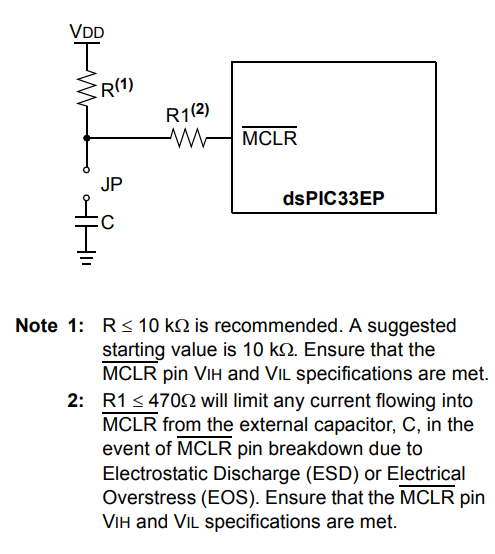
\includegraphics[width=.6\linewidth]{pictures/MCLR.PNG}
    \caption{Conexión del pin MCLR \textbf{INSERTE CITA AQUÍ}.}
    \label{fig:CAMBIAR!!!!!!!!!!}
    \end{figure}
    
    En este proyecto se ha decidido no incluir el \texit{jumper} sugerido para conexión del pin MCLR y por lo tanto $R_1$ no se añade en el diagrama esquemático.
    
    Teniendo en cuenta lo anteriormente mencionado, el conexionado final del puerto de programación mediante sonda es el siguiente:
    
    \begin{figure}[H]
    \centering 
    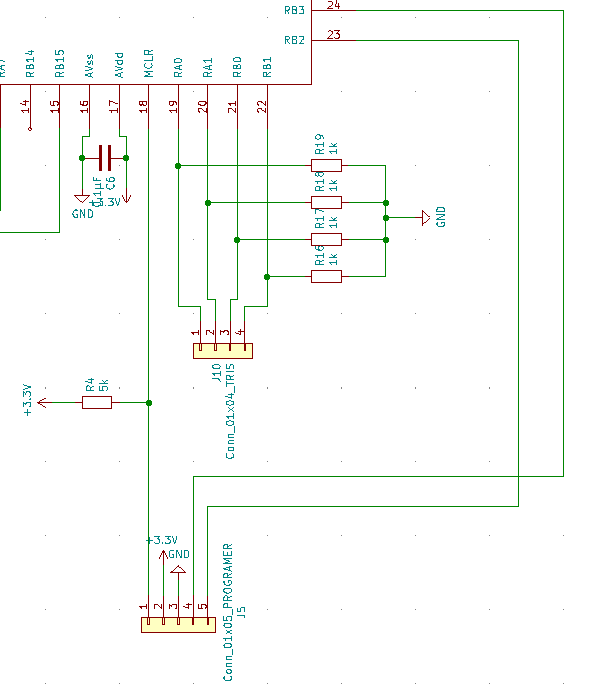
\includegraphics[width=.5\linewidth]{pictures/sonda.PNG}
    \caption{Diagrama esquemático del puerto de programación.}
    \label{fig:CAMBIAR!!!!!!!!!!}
    \end{figure}
    
    \item Puerto TRIS:  Para detectar si el brazo robótico se encuentra en uno de sus finales de carrera o zonas límite de movimiento se utilizan unos micro-interruptores que, al ser presionados por el manipulador, realizan un cortocircuito. Mediante este cortocircuito y dado que estos micro-interruptores se encuentran conectados a los pines 19, 20, 21 y 22 del microcontrolador, se puede realizar la lectura de dichos pines y detectar el estado de micro-interruptor. De esta manera, se consigue saber cuándo el manipulador ha alcanzado o no un final de carrera.
    
    A continuación se muestra un esquema de lo mencionado anteriormente:
    
    \begin{figure}[H]
    \centering 
    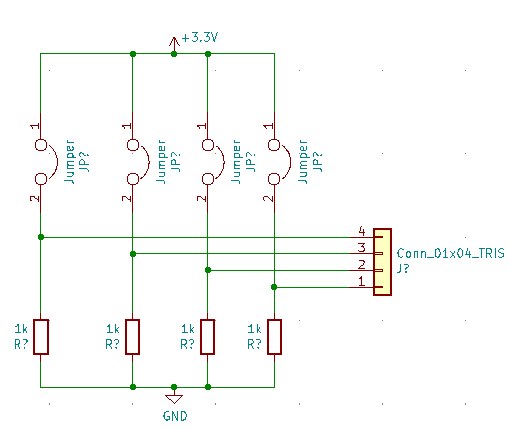
\includegraphics[width=.64
    \linewidth]{pictures/MicroSwitchesSchematic.PNG}
    \caption{Circuito lógico para los finales de carrera.}
    \label{fig:CAMBIAR!!!!!!!!!!}
    \end{figure}
    
    Mediante el conexionado anterior, si el micro-interruptor está abierto, se recibe un nivel bajo por el pin del microcontrolador; mientras que si el micro-interruptor está cerrado se recibe un nivel alto por el pin del microcontrolador. 
    
    Cabe destacar que tanto la resistencia \textit{pull-down} como la conexión a tierra se incluyen en la PCB. Sin embargo, los micro-interruptores y su conexión a $VDD$ se encuentran localizados en la estructura del brazo robótico. 
    
    El diagrama esquemático que implementa esta funcionalidad es el siguiente:
    
    \begin{figure}[H]
    \centering 
    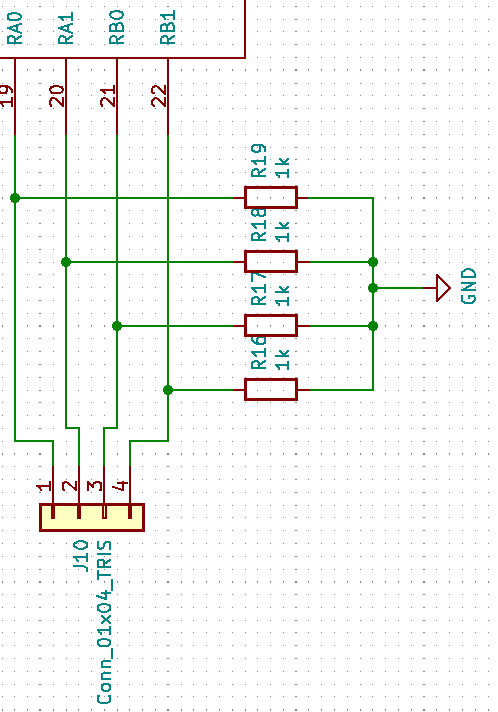
\includegraphics[width=.4\linewidth]{pictures/TRIS.PNG}
    \caption{Diagrama esquemático del puerto TRIS.}
    \label{fig:CAMBIAR!!!!!!!!!!}
    \end{figure}
    
    \item Puerto PWM: Dado que en este proyecto se realiza control de servomotores, es completamente necesario el uso de señales PWM para controlar la posición angular de los mismos y se considera a este periférico como uno de los más relevantes.
    
    Los generadores de señal PWM de este microcontrolador poseen las siguientes características técnicas relevantes:
    \begin{itemize}
        \item El microcontrolador ofrece 6 generadores de señal PWM de alta precisión y velocidad.
        \item Cada uno de los generadores posee un registro de 16 bits para la selección de la duración del ciclo de trabajo; este registro está divido en parte alta y parte baja.
        \item Es posible utilizar de forma independiente la parte alta y parte baja de cada uno de los generadores, consiguiendo de esta forma dos subgeneradores que producen señales PWM independientes. Sin embargo, su precisión se reduce a 8 bits.
    \end{itemize}
    
    El esquema mostrado por el fabricante para los generadores PWM es el siguiente:
    
    \begin{figure}[H]
    \centering 
    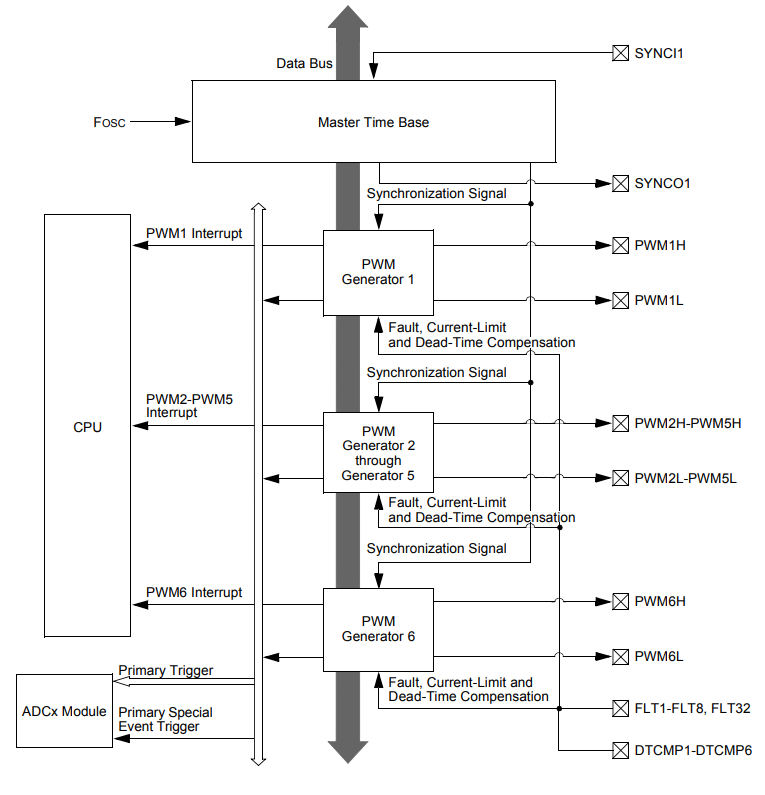
\includegraphics[width=.6\linewidth]{pictures/PWMdatasheet.PNG}
    \caption{Esquema del generador PWM \textbf{INSERTE CITA AQUÍ}.}
    \label{fig:CAMBIAR!!!!!!!!!!}
    \end{figure}
    
    Puesto que para este proyecto únicamente se necesitan cuatro generadores PWM, se ha decidido utilizar cuatro módulos con precisión de 16 bits. En el caso de utilizar la precisión completa de cada generador, la señal de salida se proporciona por el pin correspondiente a la parte baja del registro. Mediante la información obtenida del \textit{pinout} del microcontrolador, se tiene que los generadores de PWM 1, 4, 2 y 3 tienen asignados los pines 15, 13, 11 y 9, respectivamente.
    
    El conexionado final del puerto PWM en el diagrama esquemático es el siguiente:
    
    \begin{figure}[H]
    \centering 
    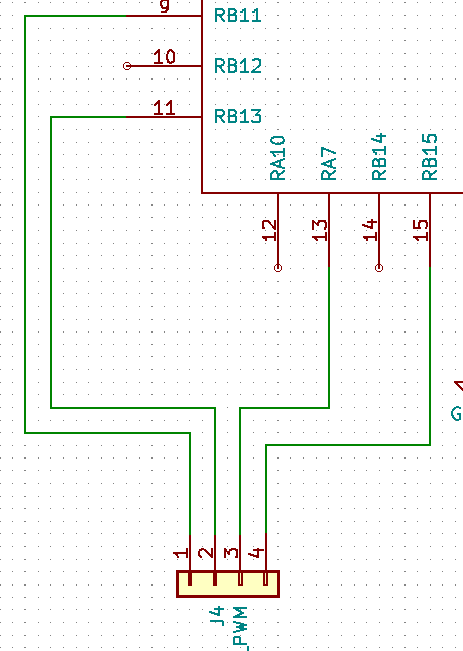
\includegraphics[width=.45\linewidth]{pictures/PWM.PNG}
    \caption{Diagrama esquemático del puerto PWM.}
    \label{fig:CAMBIAR!!!!!!!!!!}
    \end{figure}

    \item Puertos UART: Mediante el periférico UART se pueden establecer un canal de comunicación \textit{hardware} asíncrono en el cual existen diversas configuraciones en cuanto a formato de transmisión de bits y velocidades de comunicación. Suele ser un método de comunicación muy usado en microcontroladores y dispositivos \textit{hardware} en general. El protocolo UART utiliza un puerto con tres conexiones: emisor ($TX$), receptor ($RX$) y $GND$.
    
    El esquema simplificado de este periférico en el \textit{datasheet} es el siguiente:
    
    \begin{figure}[H]
    \centering 
    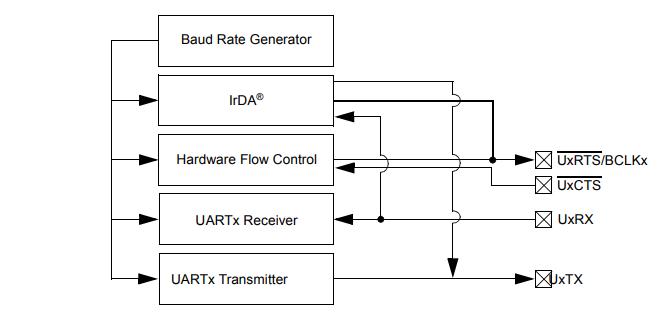
\includegraphics[width=.6\linewidth]{pictures/UARTdatasheet.PNG}
    \caption{Esquema del periférico UART \textbf{INSERTE CITA AQUÍ}.}
    \label{fig:CAMBIAR!!!!!!!!!!}
    \end{figure}
    
    Se ha tomado la decisión de incluir dos puertos UART independientes en la PCB que se ha desarrollado, con el objetivo principalmente de dedicar uno de los canales a envío y recepción de instrucciones; mientras que el otro se usa para realizar labores de depuración y pruebas.
    
    El conexionado de los puertos UART  se realiza mediante pines reconfigurables del microcontrolador, en este caso se han utilizado los pines 2 y 3 para el primer canal; además de los pines 3 y 4 para el segundo canal. El diagrama esquemático final es el siguiente:
    
    \begin{figure}[H]
    \centering 
    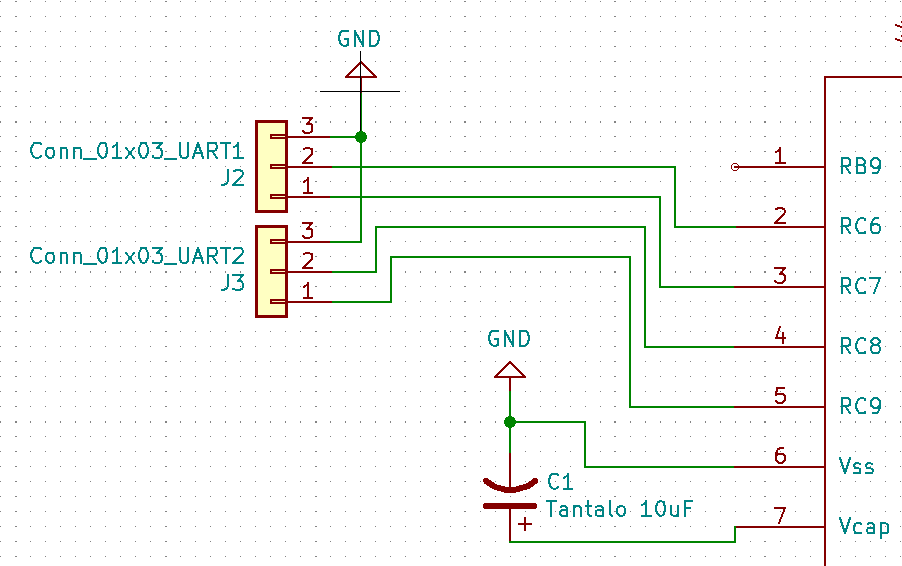
\includegraphics[width=.6\linewidth]{pictures/UART.PNG}
    \caption{Diagrama esquemático de los puertos UART.}
    \label{fig:CAMBIAR!!!!!!!!!!}
    \end{figure}
    
    
    \item LEDs de estado: se trata de tres diodos LED que se utilizan para indicar el estado del brazo robótico y demás aspectos del sistema. 
    
    Su conexionado es realizado utilizando los pines reconfigurables 41, 42 y 43, los cuales pueden ser usados para habilitar una salida digital. Se considera que un nivel alto enciende el LED mientras que un nivel bajo lo mantiene apagado.
    
    A continuación se muestra el diagrama esquemático del circuito:
    
    \begin{figure}[H]
    \centering 
    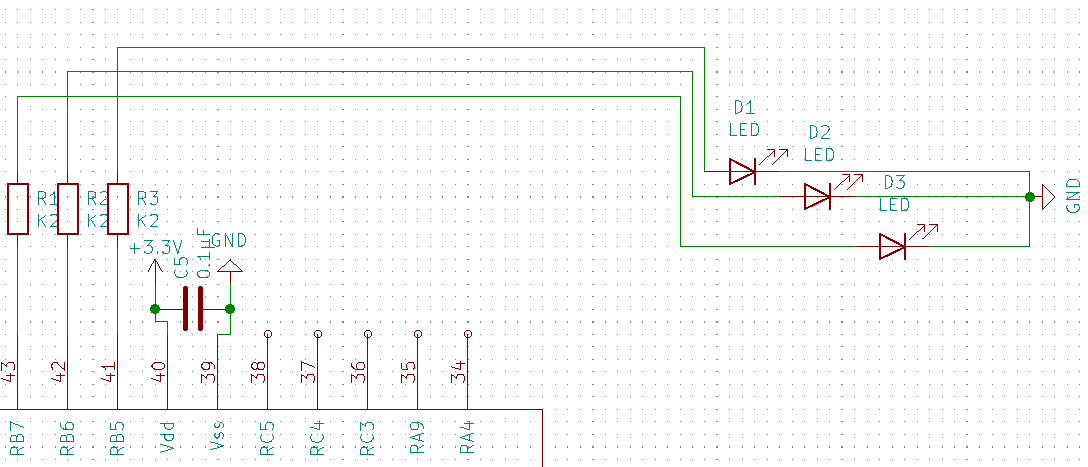
\includegraphics[width=.75\linewidth]{pictures/LEDS.PNG}
    \caption{Diagrama esquemático de los LEDs.}
    \label{fig:CAMBIAR!!!!!!!!!!}
    \end{figure}

    Teniendo en cuenta que la corriente máxima suministrada por el microcontrolador es de $18mA$ para salida digital y el que voltaje elegido ha sido $3.3V$, el pin suministraría como mucho una potencia de $0.0594W$. Se ha decidido que una potencia adecuada a suministrar sería un 80\% de la máxima, es decir $0.0475W$. Para cumplir esta restricción, se ha calculado el valor ideal de la resistencia del esquema anterior y su valor recomendado es de entre $180 \Omega$ y $200 \Omega$.
    
\end{itemize}

En conclusión, una vista completa sobre el diagrama esquemático del proyecto es la siguiente:

    \begin{figure}[H]
    \centering 
    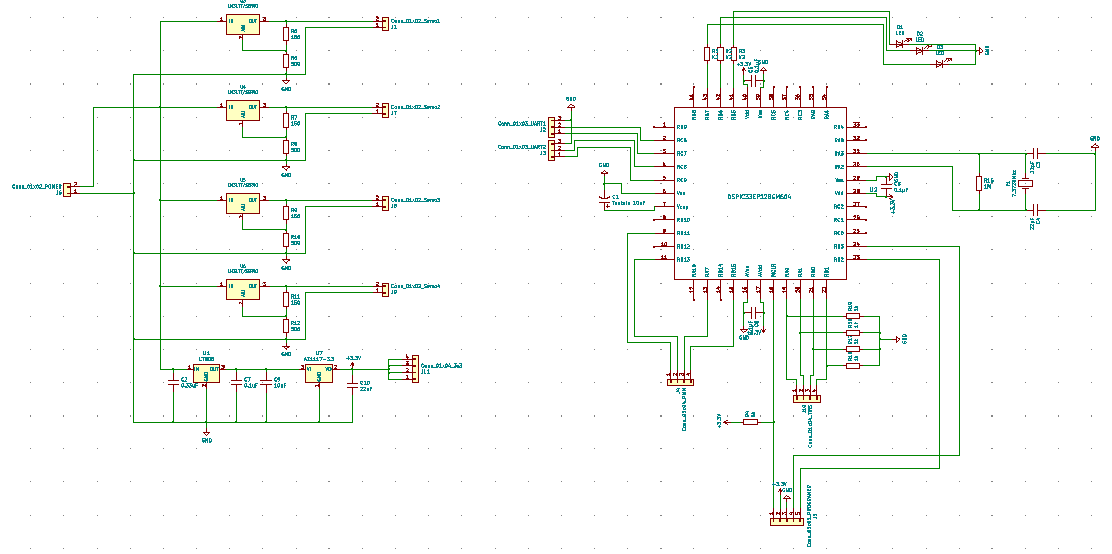
\includegraphics[width=\linewidth]{pictures/EsquematicoCompleto.PNG}
    \caption{Diagrama esquemático completo.}
    \label{fig:CAMBIAR!!!!!!!!!!}
    \end{figure}

\subsection{Conversión del diagrama esquemático a diagrama físico}

Tal y como se ha descrito en el apartado anterior, el diseño lógico de la PCB se implementa mediante el diagrama esquemático, y su objetivo es el de describir las huellas y conexiones lógicas de los componentes; sin embargo, este diseño es de alto nivel y no es implementable directamente en términos físicos. 

El siguiente paso tras completar el diagrama esquemático es transformar este diseño lógico en un diseño físico más cercano a la implementación real. 

El diseño físico de una PCB debe ser obtenido directamente de la información establecida en el diseño lógico y, por lo tanto, se tiene que transformar el diagrama esquemático en un diagrama físico, en el cual se deben contemplar los aspectos físicos de los componentes y sus conexiones, además de sus aspectos lógicos.

El objetivo principal del diseño y diagrama físico es el de plasmar la realidad física de los componentes y sus conexiones a partir de un diagrama esquemático, en el cual no se contemplan los aspectos físicos para simplificar el diseño inicial. En general, el diseño y diagrama físico es más complejo y difícil de comprender. Por ello, normalmente la primera etapa del diseño comienza con el diseño lógico y diagrama esquemático.

En general, el proceso que se debe llevar a cabo para obtener el diagrama físico a partir de un diagrama esquemático consta de varios pasos:
\begin{itemize}
    \item Asignación de huellas físicas a cada uno de los componentes lógicos.
    \item Generar un listado de redes en el cual se especifiquen las conexiones que existen entre todos los componentes.
    \item Importar ambos elementos anteriores a la herramienta de creación del diagrama físico y comenzar el diseño.
\end{itemize}

Tal y como se ha mencionado anteriormente, en primer lugar se debe asignar una huella física a cada uno de los componentes lógicos del diagrama esquemático. Este proceso se realiza en la herramienta \textit{Schematic Layout Editor} incluida en KiCad, utilizando la opción de ``asignar huellas a símbolos del sistema'' disponible en la barra de herramientas situada en la parte superior de la ventana:

\begin{figure}[H]
\centering 
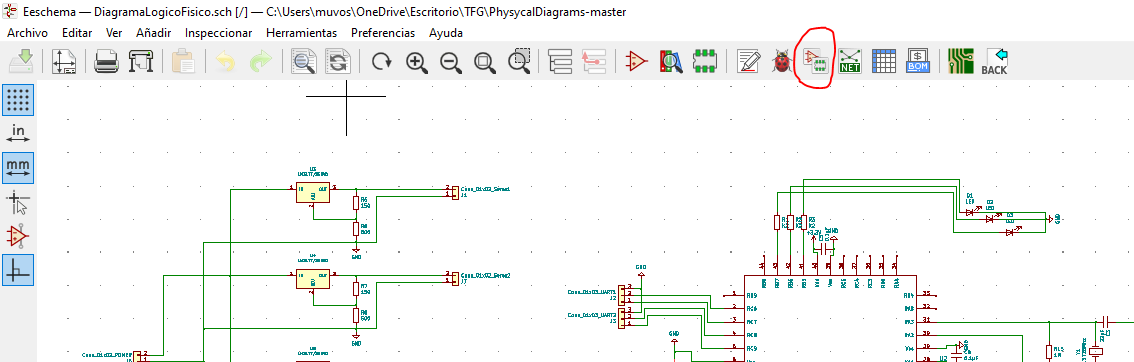
\includegraphics[width=\linewidth]{pictures/HerramientaHuellas.PNG}
\caption{Herramienta de asignación de huellas.}
\label{fig:CAMBIAR!!!!!!!!!!}
\end{figure}

Accediendo al menú de dicha herramienta, se encuentra una lista de los componentes del diagrama esquemático a los cuales se les debe asignar una huella física. Las huellas físicas que se deben asignar a cada componente lógico pueden ser seleccionadas de las extensa librerías que ofrece KiCad, o bien, ser diseñada y personalizada por el usuario.

\begin{figure}[H]
\centering 
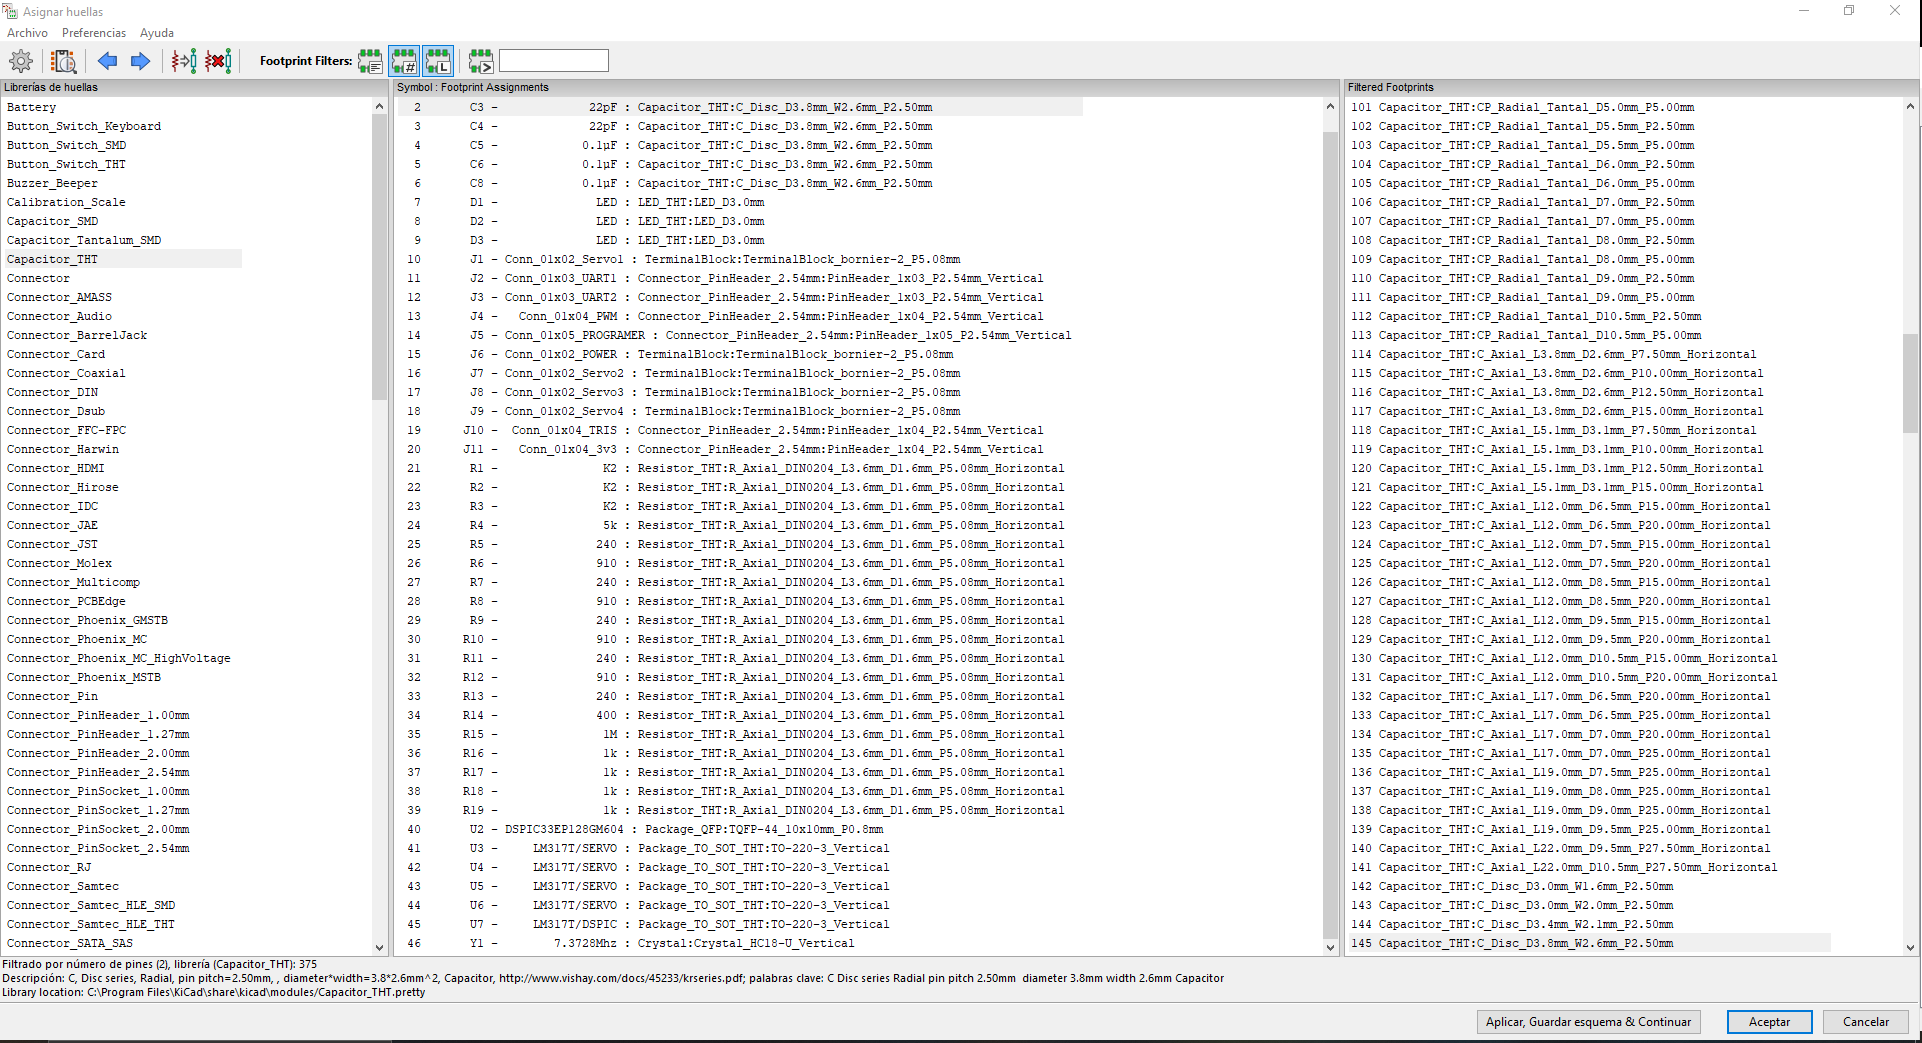
\includegraphics[width=\linewidth]{pictures/AsignarHuellaTriple.PNG}
\caption{Ventana de asignación de huellas físicas}
\label{fig:kdiagram}
\end{figure}

En la imagen anterior se muestra la ventana de asignación de huellas, la cual está dividida en tres secciones:
\begin{itemize}
    \item La sección izquierda muestra las librerías de componentes de KiCad.
    \item La sección central muestra los componentes lógicos del diagrama esquemático, seguidos de la huella física que tienen asignados.
    \item La sección derecha muestra las huellas físicas que cumplen los filtros establecidos dependiendo del componente lógico. Estos filtros suelen ser: nombre, número de pines y librería. 
\end{itemize}

Como ejemplo, en la imagen anterior se ha buscado en la librería \textit{``capacitor THT''}, ya que se quieren utilizar condensadores de agujero pasante en el diseño físico y por lo tanto, en la sección derecha de la ventana se muestran las huellas susceptibles de ser usadas, filtradas por número de pines y librería.

Una vez se ha elegido la huella que se quiere utilizar en el diseño físico, esta se asigna al componente esquemático y puede ser visualizada:


\begin{figure}[H]
\centering 
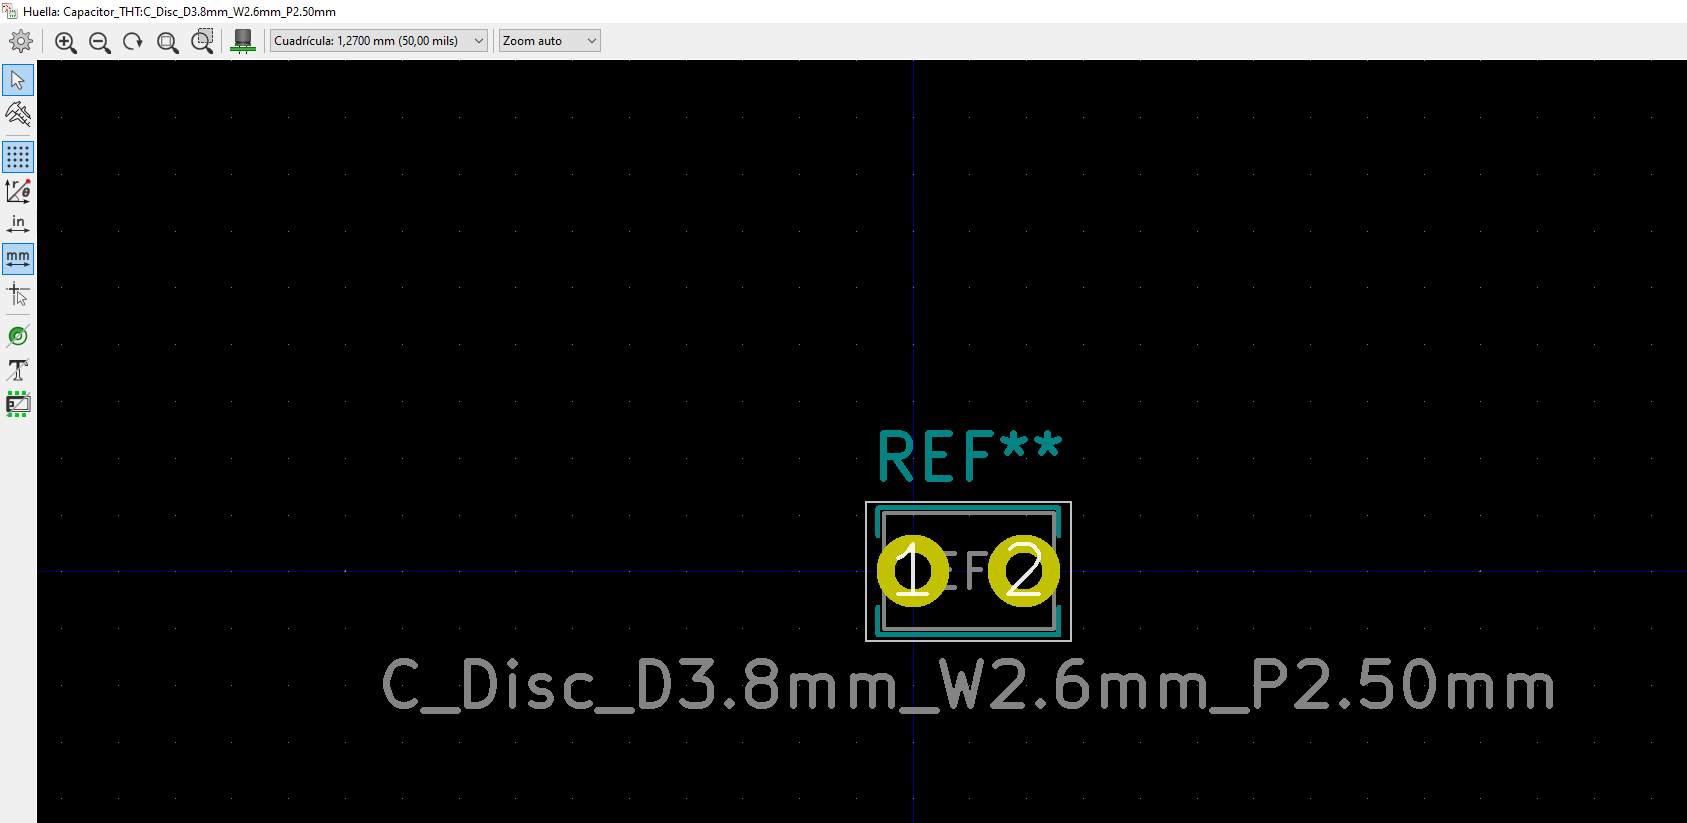
\includegraphics[width=\linewidth]{pictures/huellaCondensador.PNG}
\caption{Huella física  de un condensador usado en la PCB.}
\label{fig:CAMBIAR!!!!!!!!!!}
\end{figure}

Existen numerosos aspectos que afectan a la decisión de qué huella física asignarle a cada componente lógico y principalmente depende del tipo de implementación que se vaya a realizar en la PCB. Normalmente, estas decisiones se deben tomar a través de la información técnica suministrada por el fabricante en los diversos \texit{datasheets}.

Un ejemplo a destacar de lo recién mencionado es la huella que se ha asignado al microcontrolador dsPIC utilizado, el cual dispone de diversos encapsulados. Dichos encapsulados se muestran de forma detallada en el \texit{datasheet}.

En este proyecto, se ha decidido utilizar el encapsulado de 44 pines de soldadura superficial y de tipo ``\textit{Thin Quad Flat Package}'' (TQFP), cuya descripción en el \textit{datasheet} es la siguiente:

\begin{figure}[H]
\centering 
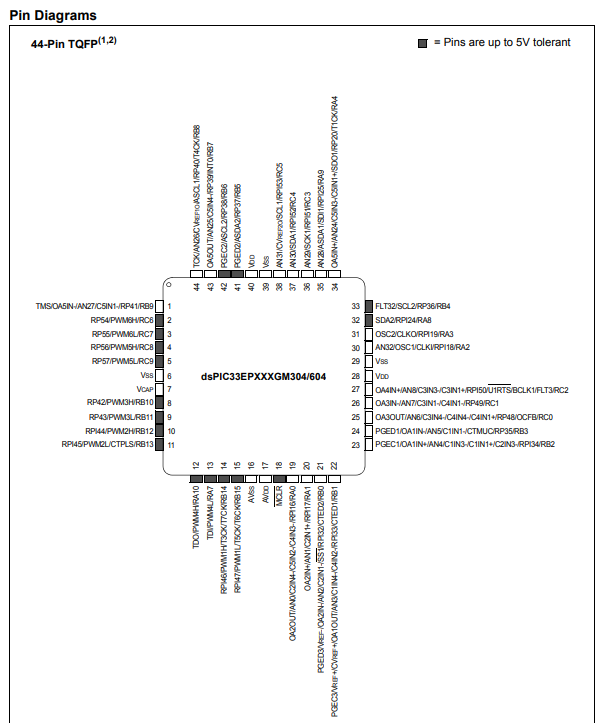
\includegraphics[width=0.9\linewidth]{pictures/TQFP.PNG}
\caption{Encapsulado elegido para el microcontrolador.}
\label{fig:CAMBIAR!!!!!!!!!!}
\end{figure}

La huella asignada al componente lógico es la siguiente y se encuentra en la librería QFP incluida por defecto en KiCad:

\begin{figure}[H]
\centering 
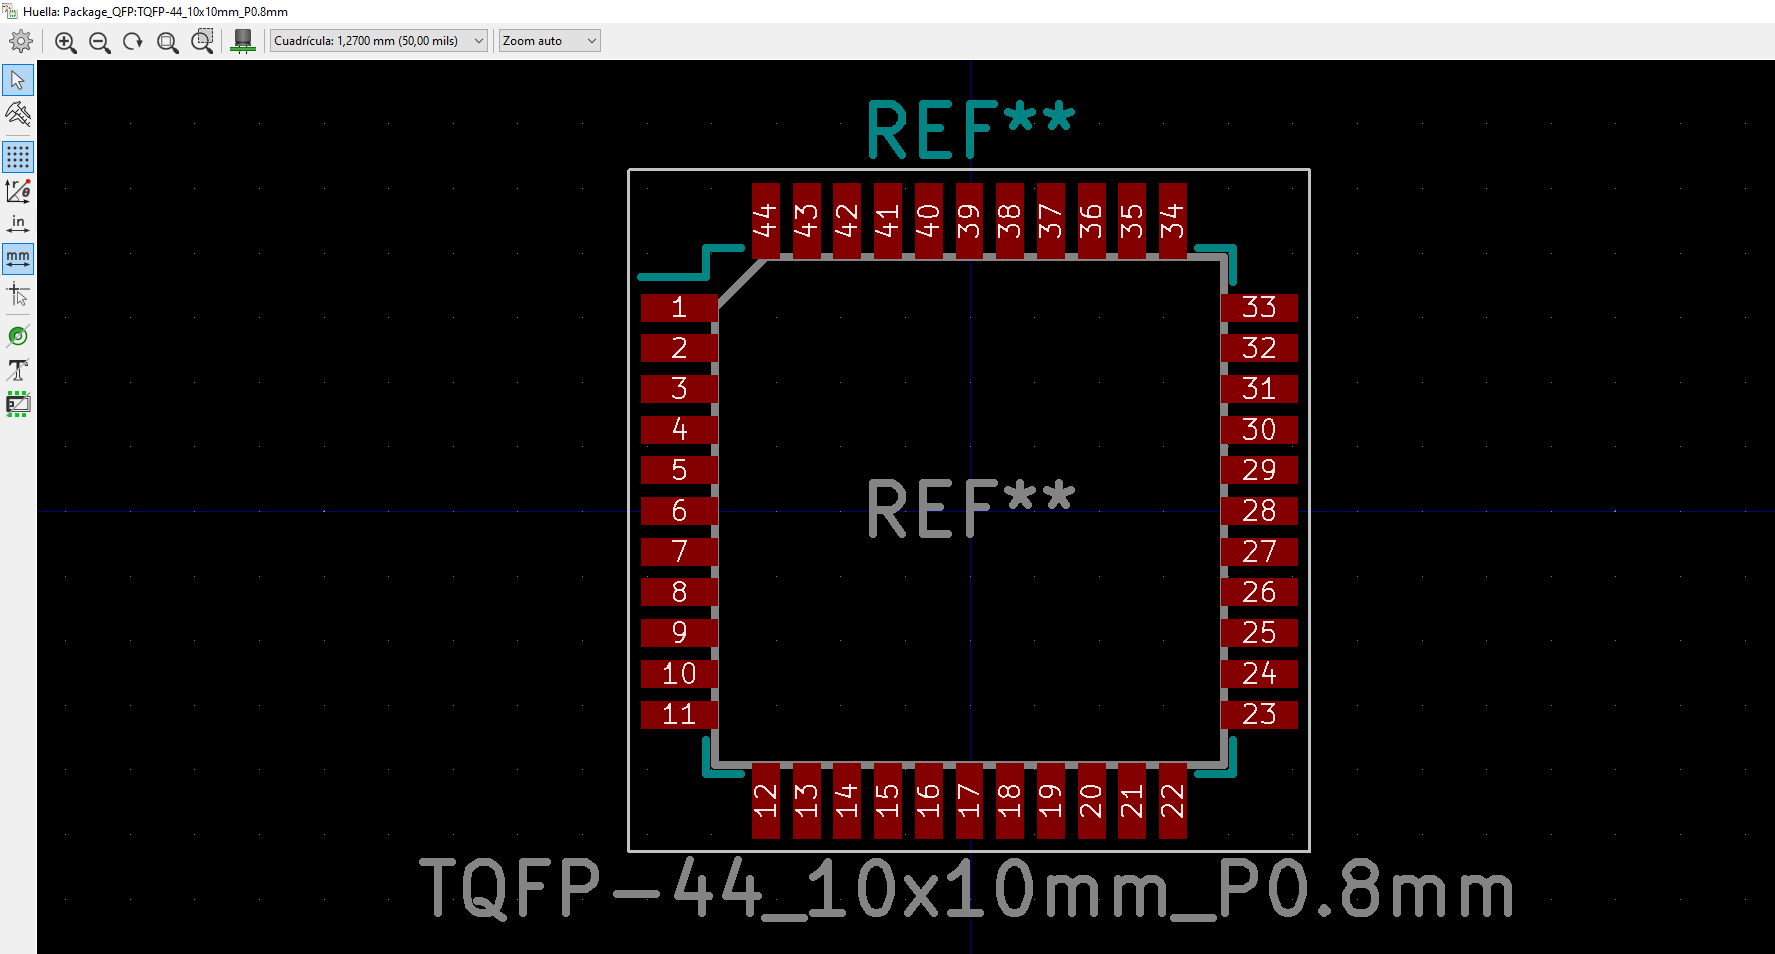
\includegraphics[width=0.9\linewidth]{pictures/HuellaPic.PNG}
\caption{Huella física asignada al microcontrolador.}
\label{fig:CAMBIAR!!!!!!!!!!}
\end{figure}

Cabe destacar que muchas de las huellas pueden ser usadas para distintos componentes de distintos fabricantes, ya que los encapsulados suelen ser similares. Sin embargo, para evitar errores, siempre se deben realizar comprobaciones con respecto a las dimensiones, número de pines, etc.

Una vez se ha realizado el primer paso, se debe generar un listado de redes de los componentes lógicos usados, sus huellas físicas asignadas y las conexiones existentes entre todos ellos. Este listado de redes se genera usando la herramienta ``Generar listado de redes'' disponible en la barra de herramientas de la parte superior de la ventana:

\begin{figure}[H]
\centering 
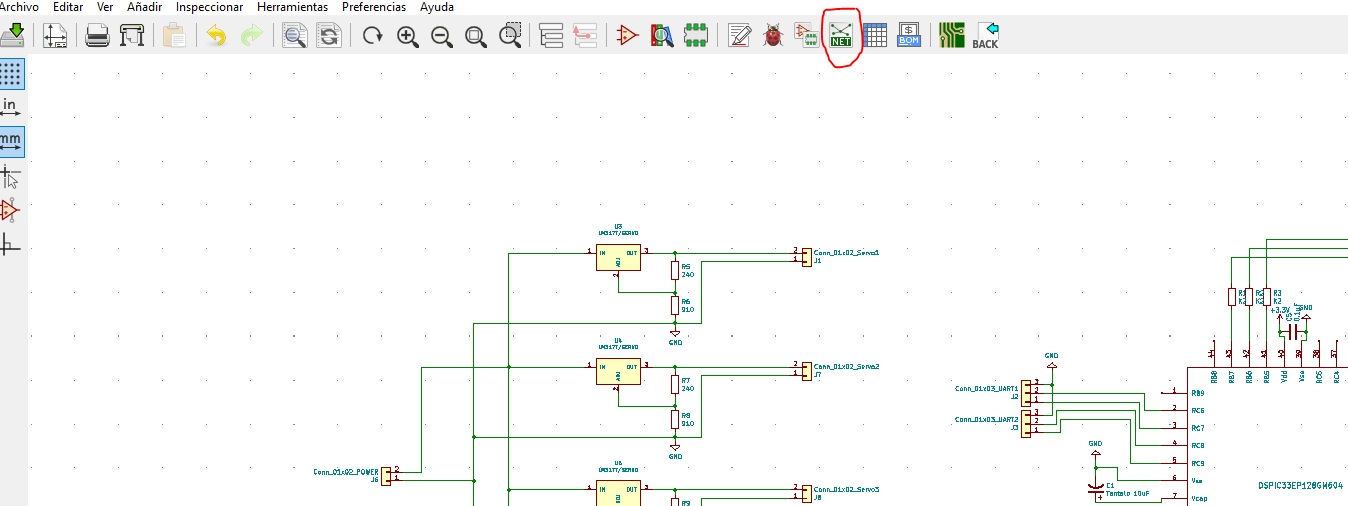
\includegraphics[width=0.9\linewidth]{pictures/GenerarRed.PNG}
\caption{Herramienta de generado de listado de redes.}
\label{fig:CAMBIAR!!!!!!!!!!}
\end{figure}

Utilizando la herramienta señalizada anteriormente se puede generar un archivo con extensión ``.net'' que almacena el listado de componentes y conexiones del diagrama esquemático. Su contenido es de la siguiente forma:

\begin{figure}[H]
\centering 
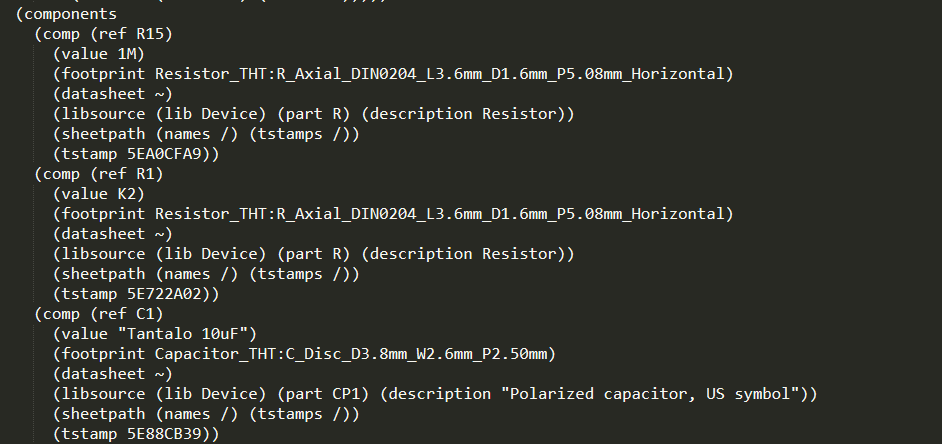
\includegraphics[width=0.9\linewidth]{pictures/net.PNG}
\caption{Archivo de listado de redes.}
\label{fig:CAMBIAR!!!!!!!!!!}
\end{figure}

Como último paso necesario para poder transformar el diagrama esquemático a diagrama físico se debe importar el listado de redes generado en el paso anterior a la herramienta de diseño físico. En este caso, la herramienta elegida ha sido ``PCBnew'' y se encuentra incluida dentro de KiCad. Esta herramienta se puede ejecutar usando la barra de herramientas de la parte superior:

\begin{figure}[H]
\centering 
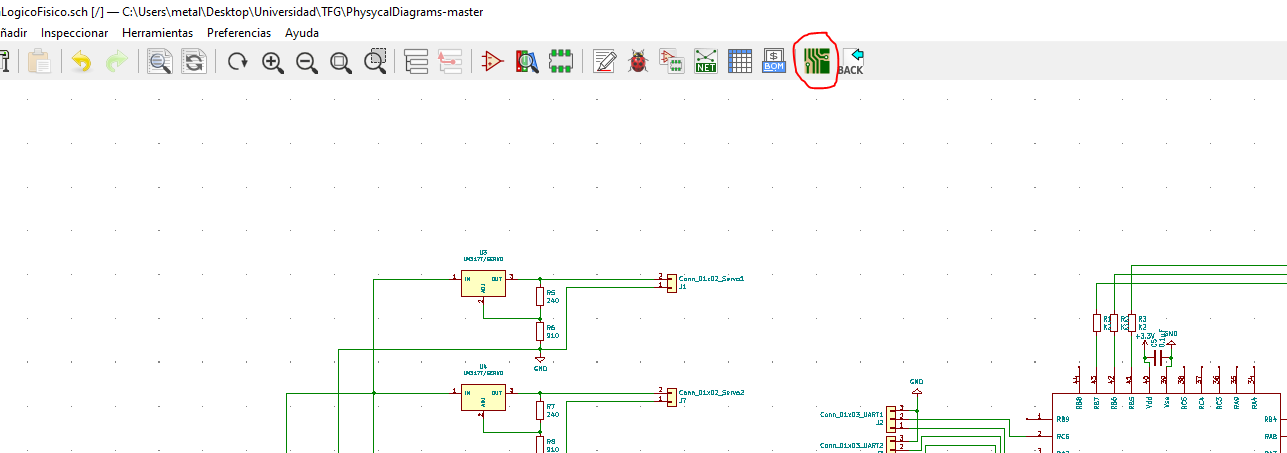
\includegraphics[width=0.9\linewidth]{pictures/PCBNEW.PNG}
\caption{Acceso directo a la herramienta ``PCBnew''.}
\label{fig:CAMBIAR!!!!!!!!!!}
\end{figure}

Una vez se ha accedido a ``PCBnew'', se debe importar el listado de redes generado anteriormente, usando el icono designado para ello en la barra de herramientas superior:

\begin{figure}[H]
\centering 
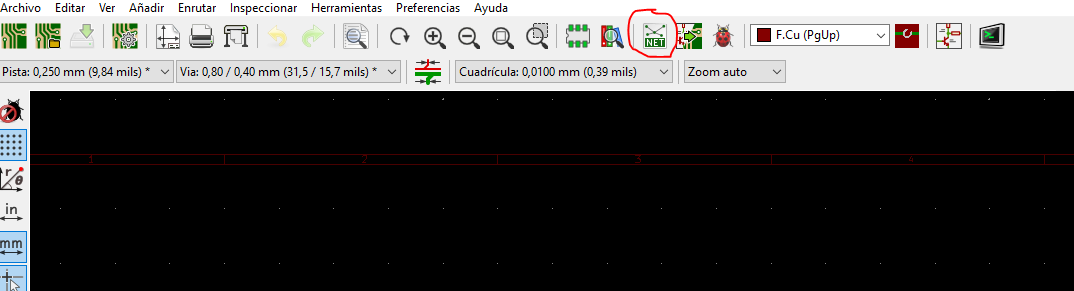
\includegraphics[width=0.9\linewidth]{pictures/redesPCB.PNG}
\caption{Herramienta de importado de listado de redes.}
\label{fig:CAMBIAR!!!!!!!!!!}
\end{figure}

Para importar el listado de redes generado anteriormente, basta con buscar la ubicación del archivo, seleccionarlo y hacer clic en ``actualizar PCB''. Al hacer esto, todos los componentes del diagrama esquemático son importados a ``PCBnew'', y su apariencia es la huella física asignada anteriormente:

\begin{figure}[H]
\centering 
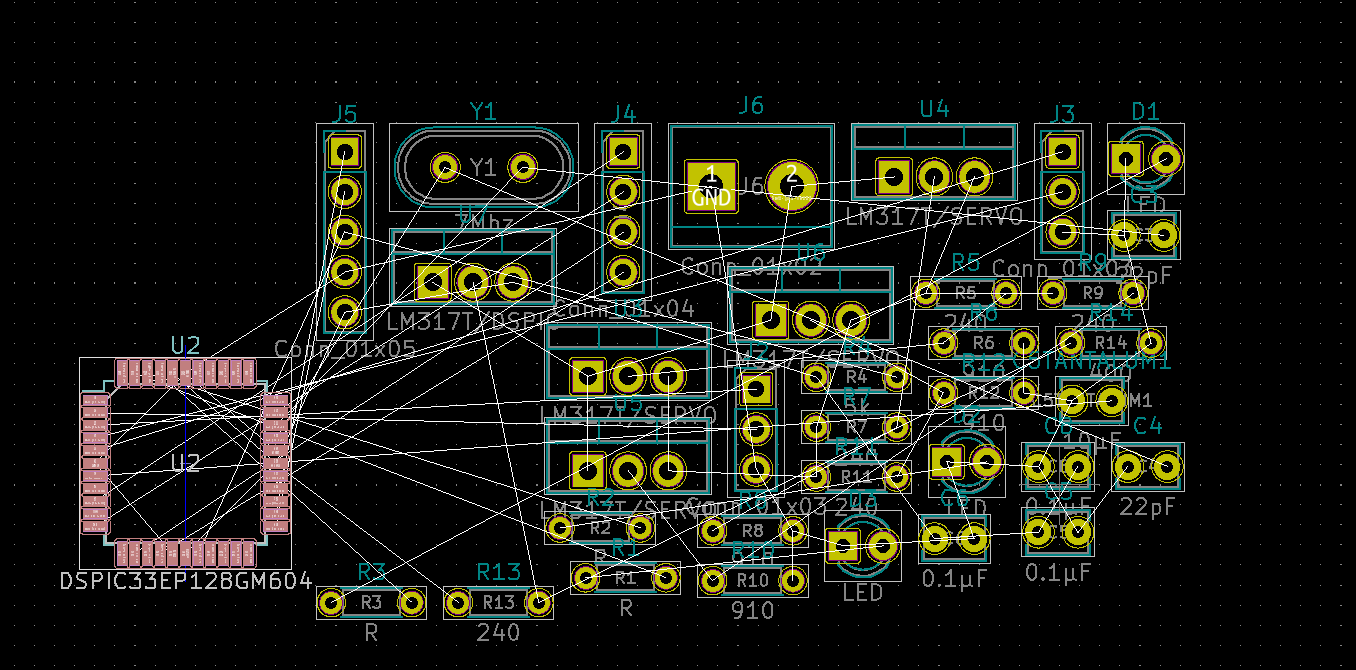
\includegraphics[width=0.9\linewidth]{pictures/bunch.PNG}
\caption{Situación inicial del diseño nada mas importar los componentes físicos.}
\label{fig:CAMBIAR!!!!!!!!!!}
\end{figure}

Inicialmente, se muestra la huella física de los componentes y sus conexiones lógica pero se encuentran desordenados. Es recomendable reorganizarlos para verificar si todos ellos han sido importados correctamente.

El primer paso para comenzar el diseño físico de la PCB es distribuir los componentes por el plano, tratando de visualizar cuál va a ser la ubicación futura de los componentes en la placa de circuito impreso y cuál van a ser las dimensiones de la misma.

\begin{figure}[H]
\centering 
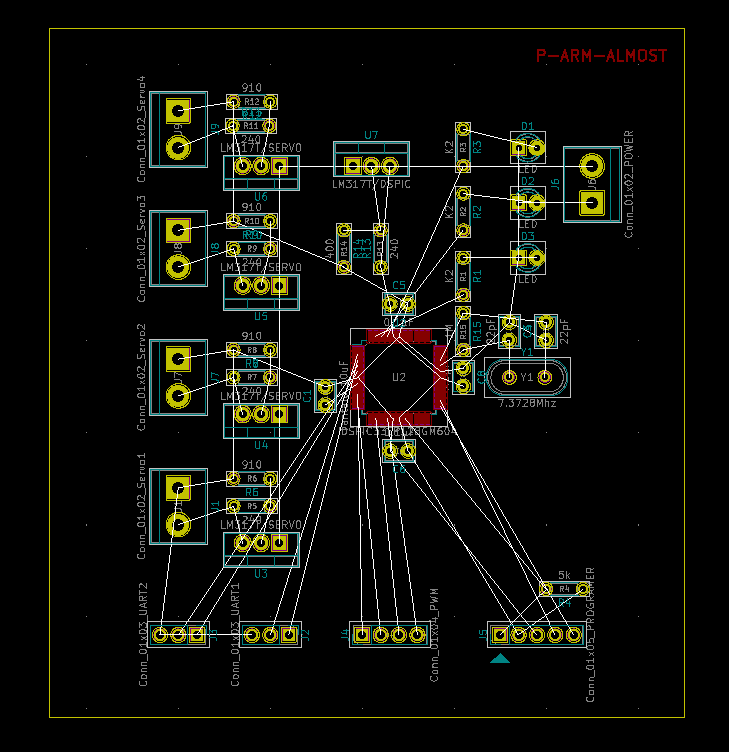
\includegraphics[width=0.9\linewidth]{pictures/DistribucionInicial.PNG}
\caption{Distribución inicial de los componentes.}
\label{fig:CAMBIAR!!!!!!!!!!}
\end{figure}

Es conveniente definir un contorno a la placa, el cual puede ser incluido en el diagrama usando la herramienta de dibujado de lineas y la herramienta de medición de distancias.

Por último, es importante remarcar que la distribución de los componentes queda a elección del diseñador de la PCB. Sin embargo, se debe de tratar de tener en cuenta factores como el tamaño deseado para la PCB, la localización de los componentes con respecto a sus conexiones cercanas, el proceso de fabricación a usar, etc.

\subsection{Conexionado de los componentes mediante pistas}
Una vez se ha creado el contorno de la PCB y se han distribuido los componentes de la forma deseada, se deben realizar las conexiones físicas entre los componentes.

Dado que se trata de una placa de circuito impreso, las conexiones lógicas entre los componentes se corresponden con pistas de cobre en el diagrama físico.

El proceso de conexionado mediante pistas se denomina ``enrutado'' y puede ser realizado de manera automática o manual. La complejidad del proceso de enrutado puede ser más o menos elevada en función del numero de componentes, capas que se utilicen para pistas, ubicación de los componentes, dimensiones de la PCB, etc. Se considera que el proceso de enrutado ha sido completado con éxito cuando todas las conexiones lógicas han sido realizadas y no existen conflictos o choques entre las pistas, así como soldaduras no realizables físicamente.

Durante el proceso de enrutado de las pistas de una PCB es habitual combinar herramientas de enrutado automático con enrutado manual, dado que, normalmente, las herramientas de enrutado automático suelen encontrar soluciones exitosas al proceso de enrutado, sin embargo no suelen ser óptimas y pueden requerir alguna modificación manual por parte del diseñador. 

En este proyecto, se ha decidido realizar un proceso de enrutado íntegramente manual, debido a que, a pesar de haber intentado utilizar la herramienta ``FreeRouting'' de enrutado automático, no se ha obtenido un resultado óptimo y era bastante complejo.

El proceso de enrutado se ha realizado utilizando ambas capas de la PCB, esto quiere decir que se han trazado pistas en la capa de soldadura y en la capa de componentes. Esta decisión se ha tomado principalmente debido a que en esta PCB se usan componentes de tipo ``THT'' (\textit{Through-Hole Technology}) y ``SMT'' (\textit{Surface-Mount technology}), por lo tanto es completamente necesario incluir pistas en la capa de componentes y capa de soldadura.

En relación con lo anterior, las dos capas mencionadas anteriormente cumplen una función específica:
\begin{itemize}
    \item La capa superior o de componentes contiene las pistas de comunicación del microcontrolador, ya que este componente es de tipo ``SMT''.
    \item La capa inferior o de soldadura contiene las pistas de alimentación de la PCB, en la cual se han realizado las soldaduras de los componentes ``THT''.
    \item Para comunicar las pistas de ambas capas se han realizado vías de conexión en los casos necesarios. Un ejemplo de su uso está en el conexionado de los pines del microcontrolador en la capa superior con las pistas de los conectores, los cuales se encuentran soldados en la capa inferior de soldadura.
\end{itemize}

Otro de los aspectos claves a la hora de enrutar una PCB, es escoger un ancho de pista adecuado. Algunos de los factores que afectan a esta decisión son los siguientes:
\begin{itemize}
    \item Intensidad de corriente y voltaje que conducirá la pista. Distinción entre pistas de alimentación y de comunicación de señales digitales.
    \item Requerimientos de tamaño de la PCB, ya sea por número de pistas, espacio disponible, tamaño de los pines de conexión de componentes, etc.
    \item Limitaciones físicas y de precisión del proceso de fabricación de la PCB.
    \item Otros factores como la resistividad del material de la pista, el aumento de temperatura máximo tolerado por la misma o su longitud aproximada, son factores determinantes para el ancho de la pista.
\end{itemize}

KiCad incluye una herramienta denominada ``PCB Calculator'' la cual permite realizar cálculos sobre diversos aspectos relacionados con la PCB, entre ellos, el ancho de pista. Esta herramienta realiza el cálculo del ancho de pistas en función de los factores mencionados anteriormente y su interfaz es la siguiente:

\begin{figure}[H]
\centering 
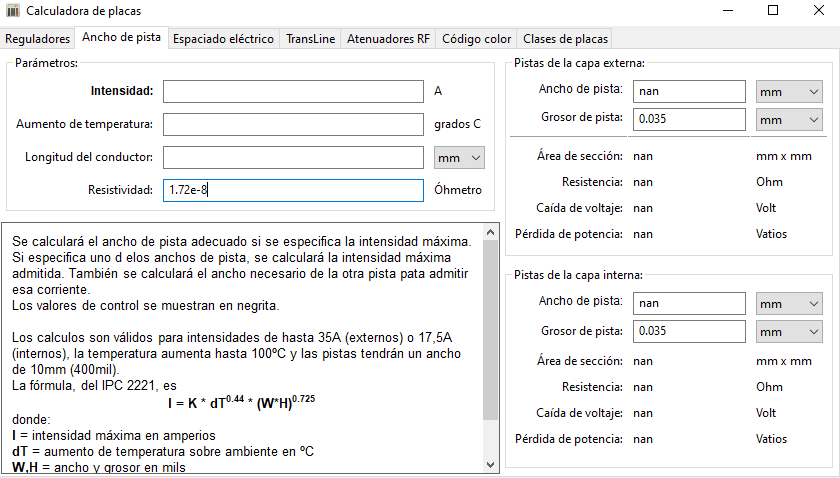
\includegraphics[width=0.9\linewidth]{pictures/PCBCalculator.PNG}
\caption{Ventana principal de ``PCB Calculator''.}
\label{fig:CAMBIAR!!!!!!!!!!}
\end{figure}

Mediante la herramienta anterior se puede realizar el cálculo para los dos tipos de pistas usadas en esta PCB: pistas de alimentación y pistas de comunicación. Para el cálculo de ambos tipos, se asume un aumento de temperatura máximo de 10 ºC, una longitud del conductor de $20cm$ y un valor de resistividad de $1.72 \cdot 10^{-8}$.

En primer lugar, se considera que las pistas de alimentación de la PCB conducen $2A$ de intensidad y un voltaje de $9V$ máximo. Teniendo en cuenta dichos datos, el ancho de pista obtenido es el siguiente:

\begin{figure}[H]
\centering 
\includegraphics[width=0.9\linewidth]{pictures/AnchoPistaAlimentación.PNG}
\caption{Cálculo del ancho de pistas de alimentación.}
\label{fig:CAMBIAR!!!!!!!!!!}
\end{figure}
 
 Se obtiene una ancho de pista de 0.78mm para las pistas de alimentación, por comodidad de aproxima este valor de ancho a 0.8mm.
 
 En segundo lugar, se considera que las pistas de comunicación del microcontrolador, conducen 0.25A y 3.3V máximo. Teniendo en cuenta dichos datos, el ancho de pista obtenido es el siguiente:
 
\begin{figure}[H]
\centering 
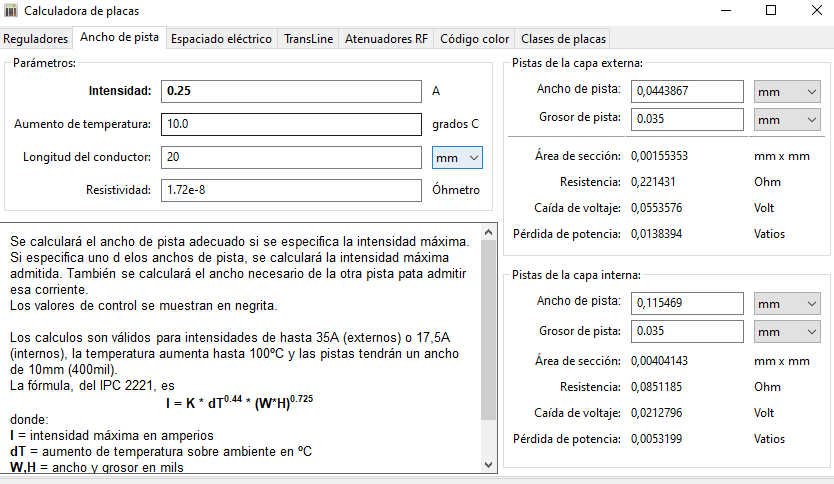
\includegraphics[width=0.9\linewidth]{pictures/AnchoPistaRestoMinimo.PNG}
\caption{Cálculo del ancho de pistas de comunicación}
\label{fig:CAMBIAR!!!!!!!!!!}
\end{figure}

Se obtiene un ancho de pista de $0.044mm$ para las pistas de comunicación, sin embargo, se ha decidido no trazar pistas con un ancho menor a $0.4mm$, debido principalmente a que se pueden producir errores en el proceso de fabricación.

En este momento, cabe destacar que el proceso de fabricación llevado a cabo para construir la placa, es de carácter artesanal, no industrial.

Asumiendo un ancho mínimo de pista de $0.4mm$, las pistas de comunicación están sobredimensionadas por motivos justificados y por lo tanto se obtiene el siguiente cálculo:

\begin{figure}[H]
\centering 
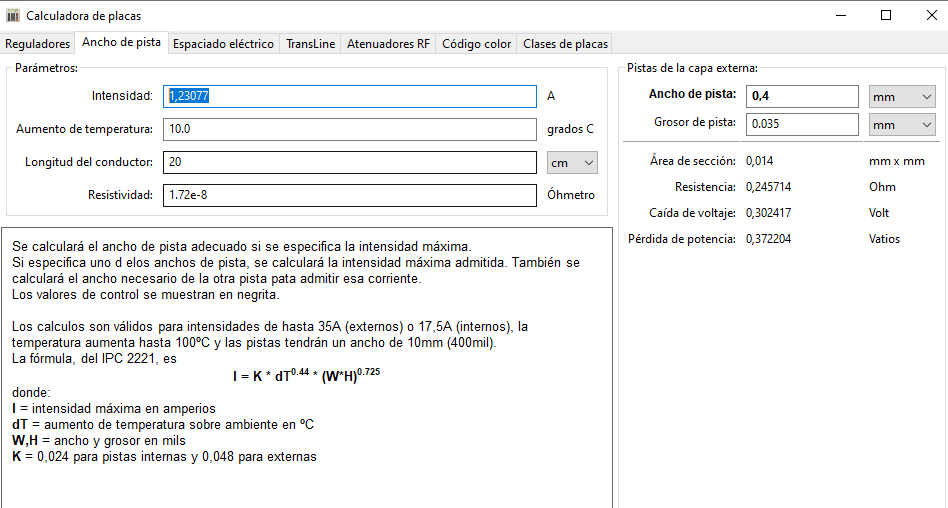
\includegraphics[width=0.9\linewidth]{pictures/AnchoPistaResto.PNG}
\caption{Cálculo inverso del ancho de pistas de comunicación.}
\label{fig:CAMBIAR!!!!!!!!!!}
\end{figure}

Las pistas de comunicación tienen finalmente un ancho de $0.4mm$ y debido a su sobredimensionado, soportan una corriente de $1.23A$, la cual se sitúa muy por encima de la corriente que circulará por las mismas.

A continuación se muestra la distribución final de los componentes físicos dentro del contorno de la PCB, aún sin haber trazado las pistas de conexión:

\begin{figure}[H]
\centering
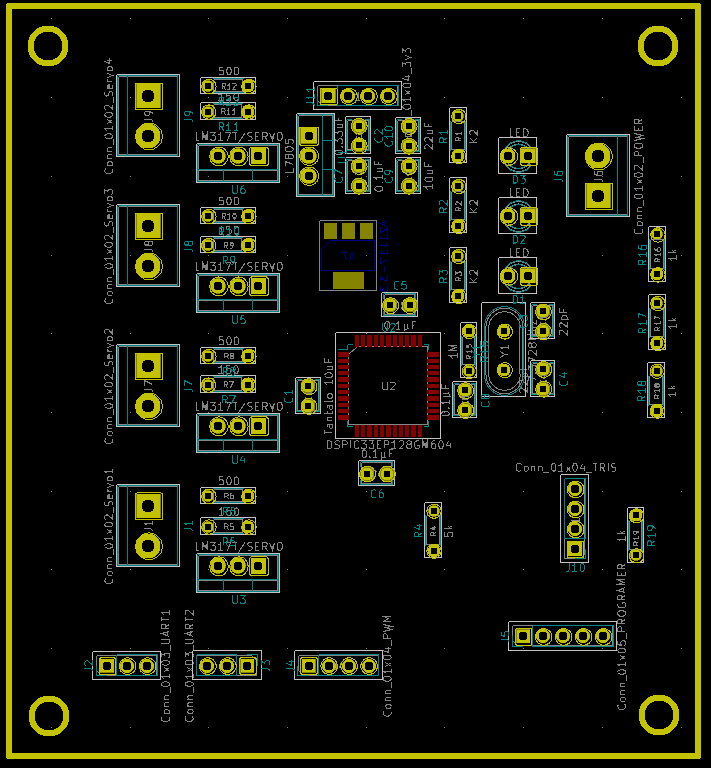
\includegraphics[width=0.9\linewidth]{pictures/DistribucionFinal.PNG}
\caption{Distribución final de los componentes físicos.}
\label{fig:CAMBIAR!!!!!!!!!!}
\end{figure}

Tal y como puede verse en la imagen anterior, las líneas blancas representan las conexiones físicas entre los componentes y por lo tanto, deben ser sustituidas por pistas de cobre. En este diagrama, se han generado conexiones inexistentes en el diagrama esquemático, ya que se contemplan conexiones físicas que a nivel lógico no son necesarias.

Tras realizar el proceso de enrutado en ambas caras, el diagrama físico final obtenido es el siguiente:

\begin{figure}[H]
\centering
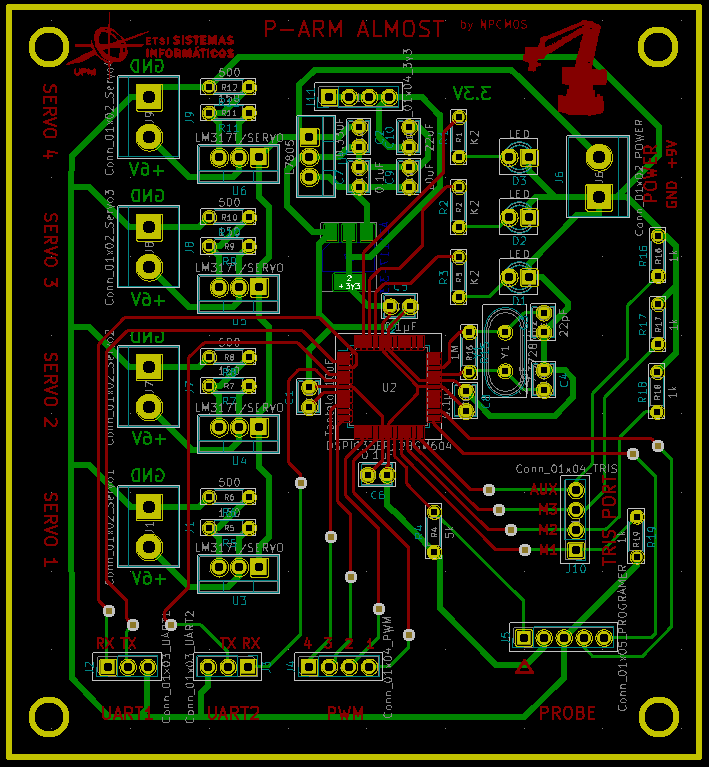
\includegraphics[width=0.9\linewidth]{pictures/PCB_FINAL_FIXED.PNG}
\caption{Diagrama físico final.}
\label{fig:CAMBIAR!!!!!!!!!!}
\end{figure}

Cabe destacar varios aspectos:
\begin{itemize}
    \item Las pistas de color rojo se corresponden con la cara frontal o de componentes.
    \item Las pistas de color verde se corresponden con la cara trasera o de soldadura.
    \item Se han incluido marcas de serigrafiado adecuadas para identificar correctamente la PCB y su interfaz.
    \item Se han incluido orificios de mecanizado para la futura sujeción de la PCB.
    \item En la parte superior izquierda y derecha de la capa frontal se han añadido los logos de la ETSISI y el \pArm{}.
    \item En la parte central de la capa frontal se ha incluido el nombre de la placa (P-ARM ALMOST) y el nombre del grupo de ingenieros (NPCMOS).
\end{itemize}

Utilizando el visualizador 3D de KiCad se puede obtener un representación cercana a la realidad de como será la PCB al fabricarse:

\begin{figure}[htbp]
    \centering
    \subfigure[Capa frontal
    %% Y ESTAS CITAS?!
    \cite{7759009FCCCDatasheetHoja}.]{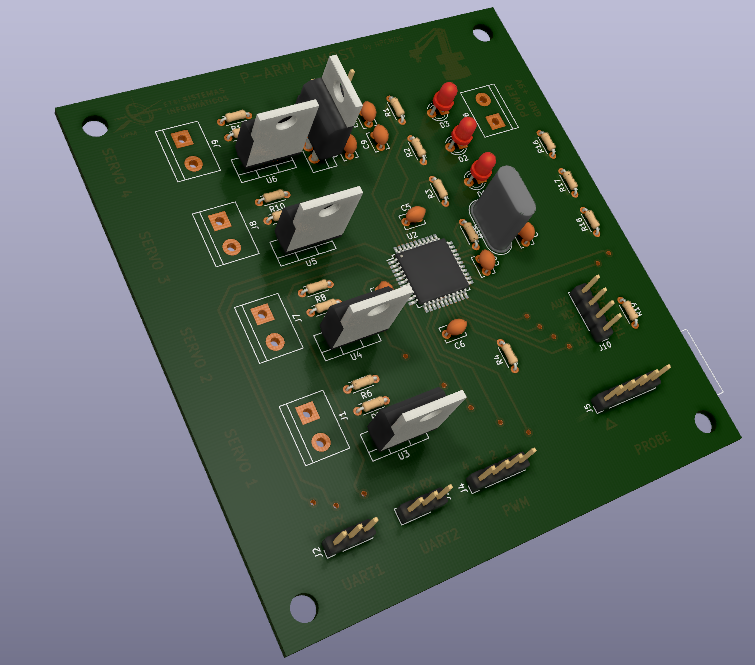
\includegraphics[width=.49\linewidth]{pictures/PlacaFinal3D.PNG}}
    \hfill
    %% Y ESTAS CITAS?!
    \subfigure[Capa trasera
    \cite{MotorCorrienteContinua2020}.]{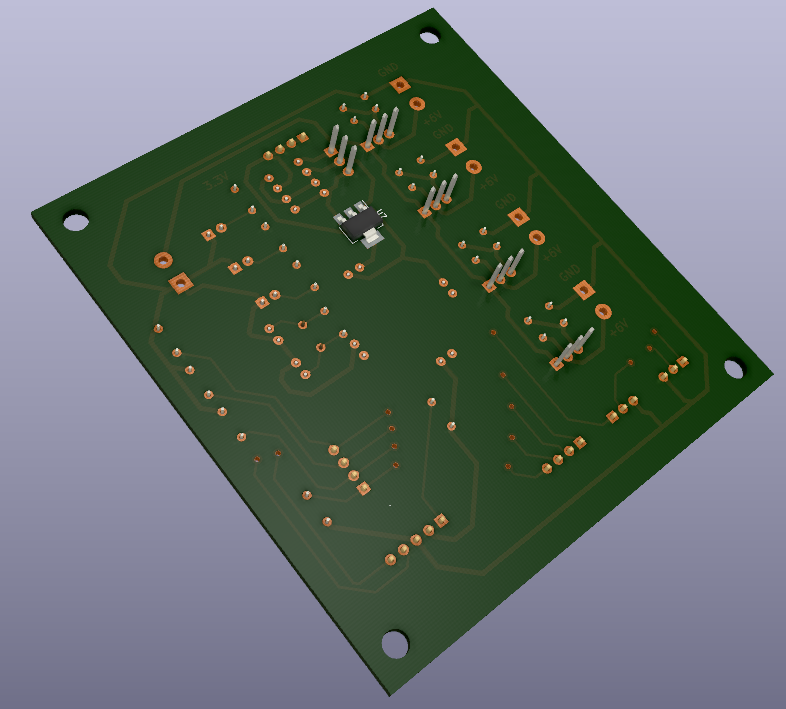
\includegraphics[width=.49\linewidth]{pictures/PlacaFinal3D2.PNG}}
    \caption{Representación 3D del diseño físico.} 
    \label{fig:lego}
\end{figure}
    
\subsection{[PENDIENTE -- J] Verificaciones realizadas al diseño lógico y físico}

El proceso de diseño de la PCB es considerado uno de los elementos críticos dentro del proyecto y por lo tanto, es necesario llevar a cabo una serie de verificaciones durante dicho proceso para minimizar el riesgo de fallos.

Dado que durante el proceso de diseño de la PCB, se han obtenido los diagramas lógico y físico, y en consecuencia, ambos son susceptibles de verificar en detalle.

En primer lugar se deben realizar las verificaciones del diseño lógico de la PCB, ya que es el primer diagrama que se realiza. Dado que el diagrama lógico aporta información de las conexiones lógicas entre los distintos componentes de la PCB, las verificaciones a realizar irán destinadas a comprobar la corrección de dichas conexiones y de los componentes empleados.

A continuación se muestra una lista de las principales verificaciones realizadas en el diagrama lógico:
\begin{itemize}

    \item Verificar si se han incluido en la PCB todos los componentes deseados.
    
    \item Verificar si se ha incluido el circuito de alimentación de la PCB, y por lo tanto, comprobar si todos los componentes están alimentados correctamente.
    
    \item Verificar si se ha incluido el conexionado mínimo recomendado por el fabricante para asegurar un correcto funcionamiento del microcontrolador y sus periféricos.
    
    \item Verificar si el conexionado de los dispositivos periféricos, puertos de conexión y demás componentes es correcto y además se ha realizado a los pines adecuados del microcontrolador.
    
    \item Verificar si se ha asignado una huella física correcta a cada uno de los componentes lógicos, la cual se utilizará posteriormente en el diagrama físico.
    
\end{itemize}

Tras realizar las revisiones anteriores en el diagrama lógico, se considera que el mismo es completamente correcto y no contienen ningún error, y por lo tanto, es susceptible de ser transformado a diagrama físico.

En segundo lugar se deben realizar las revisiones del diagrama físico, ya que se trata del diagrama que se realiza en segundo lugar. Dado que este diagrama detalla los aspectos físicos y estructurales de la PCB, las verificaciones a realizar irán destinadas a comprobar los aspectos físicos de los componentes, conexiones mediante pistas, requerimientos estructurales, dimensiones, etc.

A continuación se muestra una lista de las principales verificaciones realizadas en el diagrama físico:
\begin{itemize}
    \item Verificar que todos los componentes del diagrama lógico aparecen en el diagrama físico al importar la lista de redes.
    
    \item Verificar que todas las conexiones lógicas entre componentes del diagrama lógico aparecen representadas en el diagrama físico.
    
    \item Verificar que todas las conexiones que aparecen en el diseño físico, se corresponden con conexiones establecidas en el diagrama lógico.
    
    \item Verificar que todas las huellas físicas de los componentes lógicos son correctas y su distribución de pines es la deseada. Se debe contrastar esta información usando el datasheet de cada uno de los componentes.
    
    \item Verificar que todas las conexiones se han realizado, y por lo tanto, tienen una pista asignada.
    
    \item Verificar que todos los componentes están alimentados y que las pistas de alimentación tienen el tamaño adecuado.
    
    \item Verificar que todas las pistas de comunicación tienen el origen y destino adecuado, y que además, su ancho es el adecuado.
    
    \item Verificar que no existen pistas con un ancho menor de 0.3mm, ya que el proceso de fabricación podría fallar por debajo de este tamaño.
    
    \item Verificar que la separación mínima entre pistas es como mínimo de 0.3mm para pistas de alimentación y 0.25mm para pistas de comunicación digital.
    
    \item Verificar que no existen pistas que hagan contacto no deseado con componentes de soldadura superficial bajo su superficie.
    
    \item Verificar que se han incluido marcas de serigrafía que permitan identificar a la PCB y su interfaz de forma clara.
    
    \item Verificar que se ha incluido el mecanizado de sujeción adecuado.
    
    \item Verificar que no existan pistas que contacten con partes metálicas del mecanizado de sujeción.
    
    \item Verificar que todas las soldaduras de los componentes SMD y THT sean realizables físicamente.
    
    \item Verificar que el conector de programación dispone de espacio suficiente para realizar la conexión de la sonda.
    
    \item Verificar que las vías y pads tienen un diámetro mínimo de 1mm, con agujero de 0.5mm
    
\end{itemize}

KiCad ofrece una herramienta llamada "Comprobar reglas de diseño", la cual puede ser utilizada para facilitar el proceso de verificación del diseño físico. Utilizando esta herramienta, se pueden verificar automáticamente factores como el ancho de pista mínimo permitido, separación mínima entre pistas, conexiones no realizadas, etc. A pesar de poder realizar estas verificaciones de forma automática, se han realizado todas las verificaciones de forma manual también para reducir el riesgo de fallos.

    \begin{figure}[htbp]
    \centering
    \subfigure[Icono de verificación de reglas de diseño \cite{7759009FCCCDatasheetHoja}]{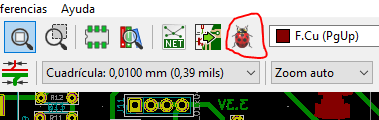
\includegraphics[width=82mm]{pictures/DRC2.PNG}}
    \subfigure[Desplegable de la herramienta
    \cite{MotorCorrienteContinua2020}]{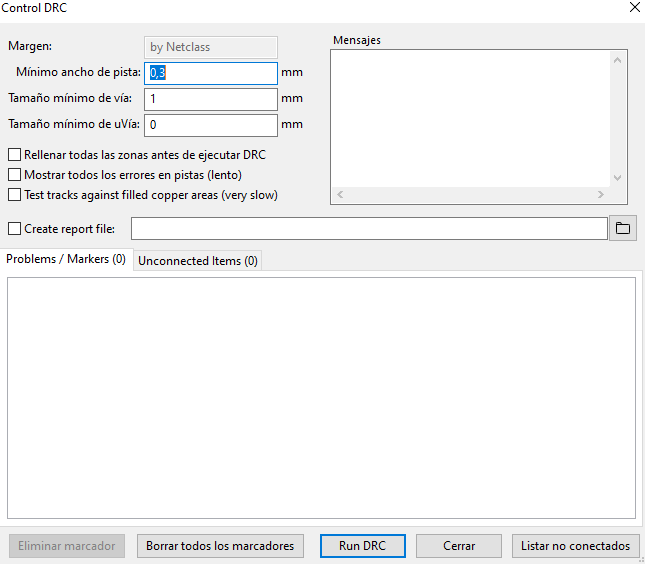
\includegraphics[width=80mm]{pictures/DRC.PNG}}
    \caption{Herramienta de verificación de reglas de diseño} \label{fig:lego}
    \end{figure}

Tras realizar todas las verificaciones anteriormente mencionadas en el diagrama físico, se han subsanado los errores encontrados previamente a realizar la fabricación de la PCB; se considera por lo tanto que el proceso de verificación del diseño ha sido exitoso.

\subsection{Construcción}

Una vez se ha finalizado el proceso de diseño de la PCB, se comienza el proceso de fabricación de la misma. Dicho proceso consta de diversas etapas, las cuales van desde la preparación de los materiales hasta la obtención del prototipo final; todas estas etapas se detallan a continuación una por una.

En primer lugar, cabe destacar que el proceso de fabricación seleccionado para construir la PCB ha sido la fotolitografía. Este proceso consiste en transferir un patrón de un circuito desde una fotomáscara a una placa de prototipado positiva mediante una serie de procesos lumínicos y químicos. Posteriormente, una vez se tiene impreso el circuito en la placa de prototipado, se puede proceder al taladrado de orificios y soldado de los componentes del circuito.

A continuación se presentan los conceptos básicos empleados durante el proceso de fotolitografía y cuyo entendimiento es fundamental para comprender el proceso de fabricación:

\begin{itemize}
    \item El proceso de fotolitografía parte necesariamente de una placa de prototipado de fibra de vidrio, la cual posee las siguientes capas de materiales:
    
    \begin{figure}[H]
    \centering 
    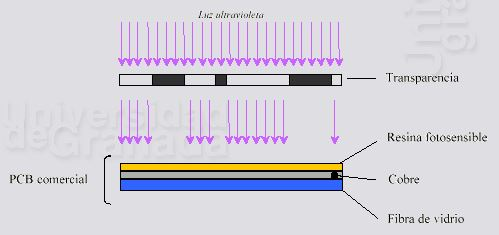
\includegraphics[width=0.9\linewidth]{pictures/Proceso1.JPG}
    \caption{Estructura de la placa de prototipado}
    \label{fig:kdiagram}
    \end{figure}
    
    Tal y como se puede ver en la imagen anterior, la placa de prototipado de fibra de vidrio posee tres capas: fibra de vidrio como material base, encima de la cual hay una capa de cobre y protegiendo la anterior, una capa de resina fotosensible a la luz ultravioleta.
    
    El aspecto clave de esta estructura en capas recae en la capa de resina fotosensible, la cual, tiene como objetivo capturar el patrón del circuito de la fotomáscara o transparencia. El funcionamiento de esta resina depende de sí la placa de prototipado es positiva o negativa:
    \begin{itemize}
        \item En las placas de prototipado positivas, la resina fotosensible que es insolada con luz ultravioleta reaccionará correctamente con el revelador, y por lo tanto desaparecerá; mientras que la resina que no es insolada permanecerá tras el revelado.
        
        \item En las placas de prototipado negativas, la resina fotosensible que es insolada con luz ultravioleta se convierte en resistente al revelador y por tanto permanecerá tras el proceso de revelado; mientras que la resina que no es insolada con luz ultravioleta, reaccionará correctamente con el revelador, y por lo tanto desaparecerá.
    \end{itemize}
    
    En este proyecto se han utilizado placas de prototipado positivas de fibra de vidrio.
    
    \item Mediante el proceso de insolado con luz ultravioleta, la fotomáscara plasma el patrón del circuito a imprimir en la resina fotosensible:
    
    \begin{figure}[H]
    \centering 
    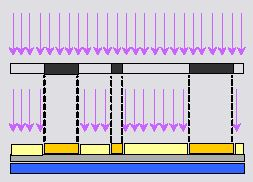
\includegraphics[width=0.65\linewidth]{pictures/Proceso2.JPG}
    \caption{Tratado de las resinas mediante insolado}
    \label{fig:kdiagram}
    \end{figure}
    
    Tal y como se puede ver en la imagen anterior, las superficies de la resina que han sido insoladas (amarillo claro), se convierten en reactivas al revelador, ya que en esa zona de la fotomáscara existe una transparencia. En las zonas en las cual la transparencia es opaca e impide el paso de la luz ultravioleta, la resina no se ve afectada y se mantiene no reactiva con el revelador.
    
    \begin{figure}[H]
    \centering 
    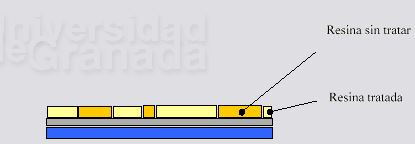
\includegraphics[width=0.8\linewidth]{pictures/Proceso3.JPG}
    \caption{Resultado tras el insolado}
    \label{fig:kdiagram}
    \end{figure}
    
    \item Mediante el proceso de revelado, se elimina la resina que fue tratada en el proceso de insolación:
    
    \begin{figure}[H]
    \centering 
    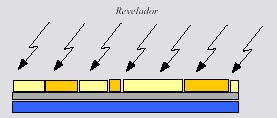
\includegraphics[width=0.7\linewidth]{pictures/Proceso4.JPG}
    \caption{Proceso de revelado}
    \label{fig:kdiagram}
    \end{figure}
    
    Tras someter la PCB al proceso de revelado, se obtiene el siguiente resultado:
    
    \begin{figure}[H]
    \centering 
    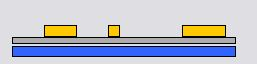
\includegraphics[width=0.7\linewidth]{pictures/Proceso5.JPG}
    \caption{Resultado tras revelado}
    \label{fig:kdiagram}
    \end{figure}
    
    Tal y como se puede ver en la imagen anterior, el proceso de revelado elimina la resina que había sido insolada, ya que se trata de una placa positiva. En estas zonas, la capa de cobre queda expuesta y sin ninguna protección. Por el contrario, en las zonas que no fueron insoladas, el revelado no actúa y por lo tanto, la resina inicial permanece protegiendo la capa de cobre.
    
    \item Mediante el proceso de atacado, se eliminan las superficies de la capa de cobre sobrantes, es decir, aquellas que no están protegidas por resina:
    
    \begin{figure}[H]
    \centering 
    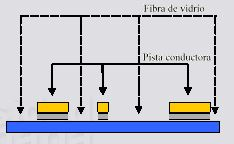
\includegraphics[width=0.6\linewidth]{pictures/Proceso6.JPG}
    \caption{Resultado tras atacado}
    \label{fig:kdiagram}
    \end{figure}
    
    Tal y como se puede observar en la imagen anterior, la capa de cobre solo permanece en los lugares que estaban protegidos por la resina inicial; este patrón coincide con el circuito de la fotomáscara. Para retirar la resina sobrante, bastan con aclarar la PCB con alcohol, quedando las pistas del circuito perfectamente delimitadas e impresas en la placa de fibra de vidrio.
    
\end{itemize}

Existen otros procesos de fabricación para PCBs que ofrecen un resultado muy parecido al deseado en este proyecto, por ejemplo fabricación mediante máquina CNC; sin embargo, por motivos de disponibilidad de materiales y maquinaria, se ha decidido utilizar la fotolitografía.

A continuación se enumeran las diversas etapas del proceso de fabricación, ordenadas cronológicamente desde el comienzo del proceso hasta su finalización:

\begin{itemize}
    \item La primera etapa del proceso de fabricación consiste en la generación de las fotomáscaras a partir del diagrama físico de la PCB.
    
    El diagrama físico representa de forma precisa cual es la apariencia física de la PCB, las huellas de sus componentes, pistas de conexión, marcas de mecanizado, serigrafía, orificios y límites. Es precisamente toda esta información la que se quiere plasmar mediante fotolitografía en la placa de prototipado positiva que contendrá el circuito impreso.
    
    Utilizando la herramienta "imprimir placa" disponible en KiCad, se puede generar las máscaras asociadas al diagrama físico:
    
    \begin{figure}[H]
    \centering
    \subfigure[Icono de impresión de placas \cite{7759009FCCCDatasheetHoja}]{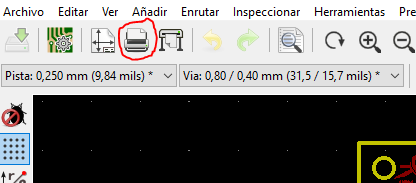
\includegraphics[width=80mm]{pictures/ImprimirPCB.PNG}}
    \subfigure[Desplegable de la herramienta
    \cite{MotorCorrienteContinua2020}]{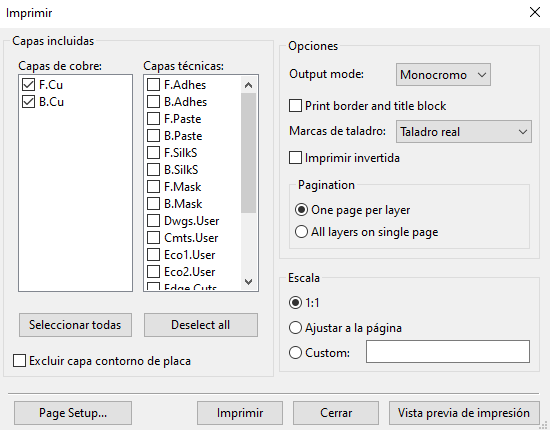
\includegraphics[width=80mm]{pictures/ImprimirPCB2.PNG}}
    \caption{Herramienta de impresión de placas} \label{fig:lego}
    \end{figure}
    
    Las fotomáscaras obtenidas tras el uso de dicha herramienta son las siguientes:
    
     \begin{figure}[H]
    \centering
    \subfigure[Máscara frontal \cite{7759009FCCCDatasheetHoja}]{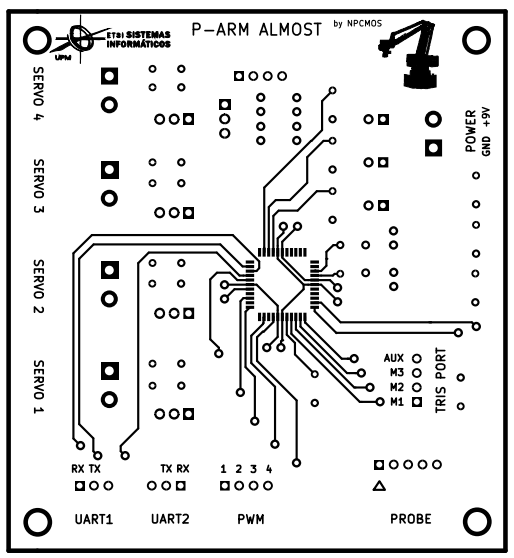
\includegraphics[width=82mm]{pictures/MascaraFrontal.PNG}}
    \subfigure[Máscara trasera
    \cite{MotorCorrienteContinua2020}]{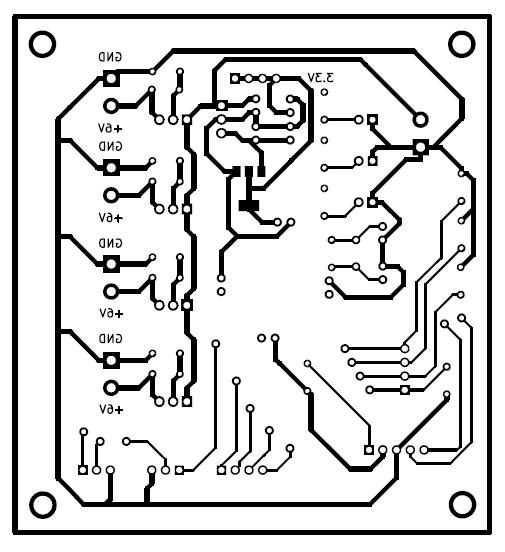
\includegraphics[width=80mm]{pictures/MascaraTrasera.PNG}}
    \caption{Fotomáscara final de la PCB} \label{fig:lego}
    \end{figure}
    
   Con el fin de poder utilizar dichas máscaras en el proceso de fotolitografía, es necesario imprimirlas en papel de transparencia, puesto que deben dejar pasar la luz en los lugares que no contienen el patrón del circuito a fotolitografiar.
   
   Para imprimir dichas máscaras en papel de transparencia, primeramente se imprimen en papel convencional y posteriormente se fotocopian a un papel de transparencia, obteniendo el resultado siguiente:
   
    \begin{figure}[H]
    \centering
    \subfigure[Máscaras de papel y sus transparencias \cite{7759009FCCCDatasheetHoja}]{\includegraphics[width=90mm]{pictures/MascarasTransparenciaPapel.jpg}}
    \subfigure[Recorte de las máscaras
    \cite{MotorCorrienteContinua2020}]{\includegraphics[width=75mm]{pictures/OperarioCortando.jpg}}
    \caption{Proceso de impresión y recorte de las fotomáscaras} \label{fig:lego}
    \end{figure}
    
     Otro de los aspectos a destacar y que es vital en relación a la impresión de las transparencias, es que, dado que todas las impresoras producen cierta distorsión en los documentos que imprimen; se debe incluir una corrección de escala XY de 1.037 para calibrar correctamente la impresión. En caso contrario, se puede producir algún pequeño desajuste en el encaje de los componentes una vez esté fabricado el circuito.
    
    Dado que el objetivo principal de dichas fotomáscaras es el de transferir el patrón del circuito de la PCB a la placa de prototipado positiva, se deben ensamblar de tal forma que permitan introducir en su interior la misma, para que posteriormente durante el proceso de insolación, se consiga fotolitografiar el circuito en ambas caras de la PCB.
    
    A continuación se muestra el ensamblado final de la funda construida con las fotomáscaras:
    
    \begin{figure}[H]
    \centering
    \subfigure[Funda de transparencias \cite{7759009FCCCDatasheetHoja}]{\includegraphics[width=60mm]{pictures/MáscaraTransparencia.jpg}}
    \subfigure[Demostración de su capacidad de contener a la placa
    \cite{MotorCorrienteContinua2020}]{\includegraphics[width=90mm]{pictures/Funda.jpg}}
    \caption{Fotomáscara final} \label{fig:lego}
    \end{figure}
    
    Cabe destacar que se han incluido dos transparencias superpuestas por cada cara de la fotomáscara para aumentar la opacidad que se genera al fotolitografiar la placa de prototipado positiva. Estas transparencias deben estar superpuestas con una exactitud extrema para impedir desfases en la impresión del circuito.
    
    
    \item En segundo lugar y una vez se ha completado el generado de la fotomáscara, se debe realizar el proceso de insolación de la placa de prototipado positiva. Durante este proceso, se realizar la transferencia del patrón del circuito desde la fotomáscara a la placa de prototipado mediante la exposición de la misma a luz ultravioleta.
    
    A continuación se muestra el proceso de insolación de la placa de prototipado positiva, el cual se ha realizado usando una maquina insoladora:
    
    \begin{figure}[H]
    \centering
    \subfigure[Placa de prototipado colocada dentro de la fotomáscara \cite{7759009FCCCDatasheetHoja}]{\includegraphics[width=75mm]{pictures/Isoladora.jpg}}
    \subfigure[Ajuste de la máquina de insolación
    \cite{MotorCorrienteContinua2020}]{\includegraphics[width=75mm]{pictures/Isoladora2.jpg}}
    \caption{Proceso de insolación de la PCB usando las fotomáscaras} \label{fig:lego}
    \end{figure}
    
    Tras el proceso de insolación, la placa de prototipado positiva habrá sido expuesta a la luz ultravioleta durante un minuto y por lo tanto, el patrón del ciruito habrá sido transferido a la superficie de resina de la placa de prototipado:
    
    \begin{figure}[H]
    \centering 
    \includegraphics[width=0.5\linewidth]{pictures/PCBisolada.jpg}
    \caption{Placa de prototipado positiva insolada}
    \label{fig:kdiagram}
    \end{figure}
    
    \item En tercer lugar y habiendo completado el proceso de insolación de la placa de prototipado, se debe llevar a cabo el proceso de revelado de la PCB.
    
    El proceso de revelado es un proceso químico mediante el cual se consigue eliminar la resina protectora de la placa de prototipado que ha sido expuesta a la luz ultravioleta durante el proceso de insolación; esta resina que es eliminada coincide con la superficie de la PCB que no contiene pistas del circuito impreso, gracias a la fotomáscara.
    
    Este proceso puede llevarse a cabo con un revelador universal indicado para realizar este tipo de labores, a continuación se muestra el usado en este proyecto:
    
    \begin{figure}[H]
    \centering 
    \includegraphics[width=0.6\linewidth]{pictures/Revelador.jpg}
    \caption{Revelador universal usado}
    \label{fig:kdiagram}
    \end{figure}
    
    El proceso de revelado de la PCB se lleva a cabo disolviendo el revelador anteriormente mencionado en agua y posteriormente, sumergiendo la PCB en esta disolución:
    
    \begin{figure}[H]
    \centering
    \subfigure[Comienzo del proceso de revelado \cite{7759009FCCCDatasheetHoja}]{\includegraphics[width=75mm]{pictures/Revelado.jpg}}
    \subfigure[Proceso de revelado en estado avanzado
    \cite{MotorCorrienteContinua2020}]{\includegraphics[width=75mm]{pictures/Revelado2.jpg}}
    \subfigure[Aclarado de la PCB
    \cite{MotorCorrienteContinua2020}]{\includegraphics[width=75mm]{pictures/Revelado3.jpg}}
    \caption{Proceso de revelado de la PCB}
    \label{fig:lego}
    \end{figure}
    
    Durante el proceso de revelado, se tienen que generar movimientos delicados de la disolución reveladora para que esta haga un efecto adecuado y consiga eliminar la resina sobrante. Cuando el proceso se ha finalizado, basta con aclarar la PCB con agua sin tocar el patrón del circuito que ha quedado revelado.
    
    \item En cuarto lugar y tras revelar el patrón del circuito de la PCB, se debe realizar el proceso de atacado.
    
   En la etapa anterior del proceso de fabricación, las zonas de la PCB que no fueron insoladas con luz ultravioleta quedan cubiertas de resina protectora; mientras que en las parte de la PCB que fueron expuestas a luz ultravioleta, la capa de cobre queda expuesta y sin cubrir por ningún tipo de resina, ya que el proceso de revelado ha eliminado dicha resina sobrante.
   
   La etapa de atacado del proceso de fabricación consiste en someter a la PCB a un proceso químico, mediante el cual se elimina el cobre de la placa de prototipado a través del atacado mediante una sal persulfato de amonio, el cual actúa de forma similar a un ácido. Las zonas de la PCB en las cuales el cobre esta expuesto, resultarán atacadas por el ácido y por lo tanto, el cobre desaparecerá. Por el contrario, las zonas de la PCB en las cuales el cobre esta protegido por una capa de resina, no serán atacadas tan agresivamente por el ácido y por lo tanto, el cobre permanecerá.
   
   Al igual que en la etapa anterior, el atacado de la PCB se realiza a través de una disolución, en este caso de agua y persulfato de amonio.
   
   A continuación se muestran algunas imágenes del proceso de atacado mediante ácido:
   
   \begin{figure}[H]
    \centering
    \subfigure[Recipiente contenedor de la disolución de atacado \cite{7759009FCCCDatasheetHoja}]{\includegraphics[width=75mm]{pictures/Atacado.jpg}}
    \subfigure[PCB siendo sometida al proceso de atacado
    \cite{MotorCorrienteContinua2020}]{\includegraphics[width=75mm]{pictures/Atacado2.jpg}}
    \caption{Proceso de atacado de la PCB}
    \label{fig:lego}
    \end{figure}
    
    Tras el proceso de atacado, el cual toma un periodo de entre una y dos horas, se debe aclarar y limpiar el circuito impreso con alcohol para eliminar los restos de resina sobrantes, así como las impurezas producidas por la disolución de atacado.
    
    Al finalizar esta etapa del proceso de fabricación, se obtiene una PCB en la cual aparece el patrón del circuito de las fotomáscaras impreso en cobre:
    
    \begin{figure}[H]
    \centering
    \subfigure[Parte frontal de la PCB \cite{7759009FCCCDatasheetHoja}]{\includegraphics[width=75mm]{pictures/Impreso.jpg}}
    \subfigure[Parte trasera de la PCB
    \cite{MotorCorrienteContinua2020}]{\includegraphics[width=85mm]{pictures/Impreso2.jpg}}
    \caption{Circuito impreso final tras el proceso de atacado}
    \label{fig:lego}
    \end{figure}
    
    \item En quinto lugar y tras realizar el proceso de fotolitografía, es recomendable realizar una revisión general de la PCB en busca de posibles imperfecciones que se hayan podido producir durante el proceso de impresión del circuito.
    
    Normalmente, durante el proceso de atacado, se pueden producir imperfecciones en el trazado de las pistas debido al que la disolución de atacado puede producir una corrosión irregular de la capa de cobre. Este tipo de imperfecciones suelen ser cortos entre pistas, fracturas de pista, etc.
    
    Para realizar el proceso de comprobación de imperfecciones, es necesario utilizar un polímetro que pueda funcionar en modo detección de cortos, para que de esta forma, se pueda determinar cuando la conductividad de las pistas es correcta. También es recomendable usar una lupa de aumento o similar para mejorar la visibilidad de las imperfecciones:
    
    \begin{figure}[H]
    \centering 
    \includegraphics[width=0.55\linewidth]{pictures/Cortos2.jpg}
    \caption{Revelador universal usado}
    \label{fig:kdiagram}
    \end{figure}
    
    \begin{figure}[H]
    \centering 
    \includegraphics[width=0.5\linewidth]{pictures/Cortos3.jpg}
    \caption{Algunos de los cortos detectados}
    \label{fig:kdiagram}
    \end{figure}
    
   En caso de encontrar algún corto entre dos pistas que no deberían estar conectadas, basta con utilizar un útil con punta para rasgar la superficie del punto de unión entre ambas.
   
   En caso de encontrar alguna fractura en una de las pistas, basta con realizar una soldadura de empalme utilizando un hilo de grapinar o similar en el punto de fractura.
   
   Ambas soluciones propuestas anteriormente son soluciones artesanales y no puede aplicarse cuando las imperfecciones son demasiado grandes o complejas de resolver, siendo mejor en este caso repetir el proceso de fotolitografía.
   
   \item En sexto lugar se debe realizar taladrado de los orificios de la PCB y el guillotinado de los márgenes de la misma.
   
   El taladrado de todos los orificios de la PCB, es decir, pads de componentes, vías y mecanizado de sujeción; se debe realizar con un taladro que cuente con una broca del tamaño adecuado, además de un soporte que aporte la estabilidad suficiente:
   
    \begin{figure}[H]
    \centering
    \subfigure[ Taladro y soporte usado \cite{7759009FCCCDatasheetHoja}]{\includegraphics[width=80mm]{pictures/Taladrado.jpg}}
    \subfigure[Taladrado de los orificios
    \cite{MotorCorrienteContinua2020}]{\includegraphics[width=80mm]{pictures/Taladrado2.jpg}}
    \caption{Taladrado de la PCB}
    \label{fig:lego}
    \end{figure}
   
   El guillotinado de la PCB se realiza con una herramienta de guillotinado que tenga precisión y permita realizar cortes limpios de la longitud necesaria. Estos cortes se realizan siguiendo los límites establecidos en el diagrama físico de la PCB.
   
   Tras el proceso de guillotinado y taladrado se obtiene el siguiente resultado:
   
    \begin{figure}[H]
    \centering 
    \includegraphics[width=0.5\linewidth]{pictures/PCBTaladrada.PNG}
    \caption{PCB con orificios taladrados y margenes guillotinados}
    \label{fig:kdiagram}
    \end{figure}
    
    \item En séptimo lugar se debe proceder a soldar el componente principal de la PCB, es decir, el microcontrolador:
    
    \begin{figure}[H]
    \centering 
    \includegraphics[width=0.5\linewidth]{pictures/DSPIC.jpg}
    \caption{Plano detallado del microcontrolador}
    \label{fig:kdiagram}
    \end{figure}
    
    Tal y como se puede ver en la imagen, el dsPic utilizado tiene un encapsulado destinado a soldadura superficial (SMD). Normalmente, los componentes SMD deben ser colocados y soldados los primeros, ya que el proceso de colocación y soldado de los mismos es delicado y requiere máxima precisión.
    
    El soldado de este tipo de componentes se realiza mediante el aplicado de una pasta de soldadura, la cual se debe colocar en el punto de contacto de los pines del componente con las pistas de cobre:
    
    \begin{figure}[H]
    \centering 
    \includegraphics[width=0.65\linewidth]{pictures/SMD2.jpg}
    \caption{Aplicado de la pasta de soldadura}
    \label{fig:kdiagram}
    \end{figure}
    
    El aplicado de la pasta de soldadura debe llevarse a cabo con la protección adecuada, ya que la pasta de soldadura es altamente tóxica.
    
    Tras aplicar la pasta de soldadura, se debe colocar el microcontrolador de forma precisa y cautelosa, cerciorándose de que cada uno de los pines realiza contacto correctamente con las pistas de la PCB:
    
    \begin{figure}[H]
    \centering 
    \includegraphics[width=0.55\linewidth]{pictures/ColocadoSMD.jpg}
    \caption{Colocado del microcontrolador sobre la pasta de soldadura}
    \label{fig:kdiagram}
    \end{figure}

    Tras colocar la pasta de soldadura, se debe introducir la PCB en un horno para que la pasta de soldadura se endurezca y selle por completo:
    
    \begin{figure}[H]
    \centering
    \subfigure[ Momento previo al horneado \cite{7759009FCCCDatasheetHoja}]{\includegraphics[width=60mm]{pictures/HORNO.jpg}}
    \subfigure[Calentado del horno
    \cite{MotorCorrienteContinua2020}]{\includegraphics[width=60mm]{pictures/HORNO2.jpg}}
    \subfigure[Horneado en curso
    \cite{MotorCorrienteContinua2020}]{\includegraphics[width=60mm]{pictures/HORNO4.jpg}}
    \subfigure[Horno a máxima potencia
    \cite{MotorCorrienteContinua2020}]{\includegraphics[width=60mm]{pictures/HORNO3.jpg}}
    \caption{Diferentes etapas del proceso de horneado}
    \label{fig:lego}
    \end{figure}
    
     Este proceso se debe realizar durante unos veinte minutos a una temperatura de entre 250º y 300º.
     
     Tras el proceso de horneado, se debe dejar enfriar la PCB. El resultado final tras el horneado es el siguiente:
     
    \begin{figure}[H]
    \centering 
    \includegraphics[width=0.55\linewidth]{pictures/POTENSIA.jpg}
    \caption{Imagen a contra luz de la PCB}
    \label{fig:kdiagram}
    \end{figure}
    
    El microcontrolador se encuentra totalmente fijado y soldado superficialmente con las pistas de conexión gracias a la pasta de soldadura. En este momento, es recomendable verificar si existen cortos entre los pines del microcontrolador, así como si la conductividad de los mismos es correcta a lo largo de las pistas:
    
    \begin{figure}[H]
    \centering 
    \includegraphics[width=0.55\linewidth]{pictures/CORTOS.jpg}
    \caption{Comprobación de cortos y conductividad de las pistas del microcontrolador}
    \label{fig:kdiagram}
    \end{figure}
    
    \item En octavo lugar, se debe realizar el soldado de las vías de conexión entre las pistas de la capa superior e inferior.
    
    Para realizar esta conexión, basta con introducir un hilo de grapinar por el orificio de la vía, realizar una pequeña soldadura con ambas pistas superior e inferior y por último, cortar el hilo excedente:
    
    \begin{figure}[H]
    \centering
    \subfigure[Vía con hilo de grapinar sin cortar \cite{7759009FCCCDatasheetHoja}]{\includegraphics[width=80mm]{pictures/Via.jpg}}
    \subfigure[Aspecto final de la vía
    \cite{MotorCorrienteContinua2020}]{\includegraphics[width=72.5mm]{pictures/VIA2.jpg}}
    \caption{Taladrado de la PCB}
    \label{fig:lego}
    \end{figure}
    
    
    \item En noveno y último lugar, se deben soldar el resto de componentes de la PCB.
    
    Los componentes restantes tienen un encapsulado de agujero pasante (THT), a excepción del regulador A1117z, el cual es de tipo SMD, sin embargo es de gran tamaño y no es necesario utilizar pasta de soldadura.
    
    Debido a lo anterior, todos estos componentes se pueden soldar de forma convencional, utilizando un soldador y estaño:
    
    \begin{figure}[H]
    \centering 
    \includegraphics[width=0.55\linewidth]{pictures/PreSoldado.jpg}
    \caption{Comienzo del proceso de soldadura}
    \label{fig:kdiagram}
    \end{figure}
    
    \begin{figure}[H]
    \centering
    \subfigure[ \cite{7759009FCCCDatasheetHoja}]{\includegraphics[width=70mm]{pictures/Soldando.jpg}}
    \subfigure[
    \cite{MotorCorrienteContinua2020}]{\includegraphics[width=72.5mm]{pictures/Soldando2.jpg}}
    \caption{Integrantes del equipo soldando componentes}
    \label{fig:lego}
    \end{figure}
    
    \begin{figure}[H]
    \centering 
    \includegraphics[width=0.45\linewidth]{pictures/PreSoldado2.jpg}
    \caption{Proceso de soldadura en curso}
    \label{fig:kdiagram}
    \end{figure}
    
    Tras finalizar el proceso de soldadura de los componentes y de haber recortado el exceso de sus pines, se obtiene el resultado final:

    
    \begin{figure}[H]
    \centering
    \subfigure[ Cara de componentes\cite{7759009FCCCDatasheetHoja}]{\includegraphics[width=70mm]{pictures/SoldaduraDelanteras.jpg}}
    \subfigure[ Cara de soldadura
    \cite{MotorCorrienteContinua2020}]{\includegraphics[width=70mm]{pictures/SoldadurasTraseras.jpg}}
    \caption{Integrantes del equipo soldando componentes}
    \label{fig:lego}
    \end{figure}
    
    Cabe destacar que tras el proceso de soldadura, se deben revisar las soldaduras en cuanto a los siguientes aspectos:
    \begin{itemize}
        \item Verificar si las soldaduras son limpias y brillantes.
        \item Verificar si las soldaduras conducen correctamente
        \item Eliminar excesos de estaño que puedan producir cortos.
    \end{itemize}
\end{itemize}

En este punto se considera que el proceso de fabricación de la PCB ha terminado, a falta de realizar el proceso de verificación que queda por realizar y que se muestra en el siguiente apartado.

\subsection{Verificaciones del prototipo construido}

Tras completar la fabricación de la PCB, es recomendable realizar algunas comprobaciones mínimas para asegurarse de que el prototipo construido es funcional:

\begin{itemize}
    \item Al completar la impresión del circuito y antes de soldar los componentes, se debe verificar la correcta conductividad de las pistas de cobre, así como la búsqueda de cortocircuitos o fracturas. Para esta labor se debe utilizar un voltímetro.
    
    \item  Posteriormente, pero antes de soldar los componentes, se debe verificar la correcta conducción de las distintas redes según lo descrito en el diagrama lógico. Para esta labor se debe utilizar un voltímetro.
    
    \item En el momento de soldar los componentes, se debe verificar su correcta inserción en los orificios de los pads; verificando también que su orientación y colocación de pines sea la correcta.
    
    \item Tras realizar todos las verificaciones anteriores y una vez se ha completado el proceso de soldadura de los componentes, se debe realizar el primer encendido del microcontrolador y el testeo de todos los componentes de la PCB.
    
        
    \begin{figure}[H]
    \centering 
    \includegraphics[width=0.55\linewidth]{pictures/PrimerEncendido.jpg}
    \caption{Primer encendido de la PCB usando un código de prueba del PWM}
    \label{fig:kdiagram}
    \end{figure}
    
    \begin{figure}[H]
    \centering 
    \includegraphics[width=0.55\linewidth]{pictures/PruebaUart}
    \caption{Prueba del funcionamiento de la UART}
    \label{fig:kdiagram}
    \end{figure}
    
    \begin{figure}[H]
    \centering 
    \includegraphics[width=0.55\linewidth]{pictures/PruebaServos.jpg}
    \caption{Prueba del funcionamiento de los servomotores}
    \label{fig:kdiagram}
    \end{figure}
    
\end{itemize}

Todas las pruebas realizadas dieron buen resultado y gracias a ellas se descubrieron alguno de los contratiempos descritos en el apartado siguiente.

\subsection{Contratiempos ocurridos y soluciones ingeniadas}

El proceso de fabricación de la PCB ha sido uno de las etapas mas críticas dentro del proyecto y por lo tanto se considera importante comentar algunos de los contratiempos que han ocurrido, puesto que estos han tenido un impacto considerable en el desarrollo del proyecto.

En general, estos contratiempos han ralentizado el proceso de fabricación, sin embargo, mediante su detección y correcta solución, se ha obtenido una PCB mucho mas robusta y segura; ya que se han revelado aspecto negativos que de otra forma habrían pasado desapercibidos.

A continuación se muestran los principales contratiempos ocurridos y las soluciones que se han llevado a cabo para enmendarlos:

\begin{itemize}
    \item El primer contratiempo sucedido durante el proceso de fabricación está relacionado con el proceso de atacado de la PCB.
    
    Tal y como se ha explicado en apartados anteriores, el proceso de atacado a la PCB, tiene como objetivo eliminar la capa de cobre  en los lugares en los cuales no debe haber circuito impreso. Este proceso se realiza mediante una disolución de persulfato de amonio, la cual reacciona con la capa de cobre de la PCB y la corroe.
    
    La efectividad de esta disolución de atacado sobre la PCB verse afectada en función de la temperatura a la que se realiza el proceso, saturación de la disolución y otros factores específicos.
    
    Debido a lo expuesto anteriormente, se realizaron dos intentos fallidos de atacado de la PCB, en los cuales la disolución no consiguió eliminar la capa de cobre de los lugares que no estaban protegidas por resina. El resultado obtenido fue el siguiente:
    
    \begin{figure}[H]
    \centering 
    \includegraphics[width=0.55\linewidth]{pictures/FalloPCB.jpg}
    \caption{PCB tras proceso de atacado fallido}
    \label{fig:kdiagram}
    \end{figure}
    
    Tras cada uno de los intentos fallidos, se tuvo que repetir el proceso de insolación de las fotomáscaras sobre una nueva placa positiva de prototipado.
    
    Después de dos intentos fallidos, se decidió desechar la disolución de atacado, ya que esta llevaba bastante tiempo fabricada y podría estar en mal; posteriormente se creo una nueva disolución de atacado:
    
    \begin{figure}[H]
    \centering 
    \includegraphics[width=0.65\linewidth]{pictures/BreakingBad.jpg}
    \caption{Proceso de creación de la disolución de atacado}
    \label{fig:kdiagram}
    \end{figure}
    
    Trás el atacado con la nueva disolución, el proceso tuvo éxito y el circuito se imprimió correctamente en la placa de prototipado.
    
    A continuación se muestran las PCB obtenidas durante esta etapa:
    
    \begin{figure}[H]
    \centering 
    \includegraphics[width=0.65\linewidth]{pictures/CursedPodium.jpg}
    \caption{Intentos de fabricación de la PCB}
    \label{fig:kdiagram}
    \end{figure}
    
    Tal y como se puede observar, en el centro de la imagen se encuentra la PCB exitosa y en los laterales los intentos fallidos, en los cuales el cobre no se eliminó adecuadamente.
    
    \item Otro de los contratiempos sucedidos fue detectado tras el proceso de soldado de los componentes, inmediatamente después de realizar el primer encendido del microcontrolador.
    
    Este contratiempo afecta al periférico PWM por partida doble, ya que se detectó una fractura en una de las pistas de comunicación del puerto PWM y a su vez, se comprobó que el modulo PWM interno que usaba esta pista también estaba defectuoso y era inservible.
    
    En la siguiente imagen se puede apreciar la fractura en la pista de cobre:
    
    \begin{figure}[H]
    \centering 
    \includegraphics[width=0.65\linewidth]{pictures/FracturaPista.jpg}
    \caption{Fractura en pista de cobre}
    \label{fig:kdiagram}
    \end{figure}
    
    En primer lugar, se procedió a realizar un parcheo de la pista usando hilo de grapinar:
    
    \begin{figure}[H]
    \centering 
    \includegraphics[width=0.65\linewidth]{pictures/Parche.jpg}
    \caption{Parcheo de la pista usando hilo de grapinar}
    \label{fig:kdiagram}
    \end{figure}
    
   Tras verificar que la conductividad del nuevo parche era correcta, se detectó que el modulo PWM seguía sin funcionar a pesar de que la fractura se había solucionado. Posteriormente a realizar algunas pruebas al respecto usando un osciloscopio, se concluyó que el módulo estaba defectuoso y no funcionaba.
   
   Para solucionar este problema, se optó por utilizar un hilo de grapinar para reconectar el puerto PWM inservible a otro de los pines del microcontrolador, el cual usaba un módulo PWM que funcionaba correctamente y que no estaba siendo usado. Se obtuvo el siguiente resultado:
   
    \begin{figure}[H]
    \centering 
    \includegraphics[width=0.65\linewidth]{pictures/HiloGrapinar.jpg}
    \caption{Reconexión del nuevo módulo PWM al puerto}
    \label{fig:kdiagram}
    \end{figure}
       
    \begin{figure}[H]
    \centering 
    \includegraphics[width=0.65\linewidth]{pictures/SoldaduraPrecisión.jpg}
    \caption{Soldadura del hilo de reconexión con el nuevo pin}
    \label{fig:kdiagram}
    \end{figure}
    Tal y como se puede observar, el reducido tamaño de la soldadura requirió que este proceso fuese realizado con máxima precisión. Además, por precaución, se eliminó parte de la pista original para evitar errores en la señal.
    
    A pesar de que esta solución es de carácter artesanal y lo recomendable hubieses sido fabricar de nuevo la PCB, se tomó la decisión de realizar este arreglo para reducir el impacto del contratiempo en el proyecto, ya que además esta solución mostró muy buen resultado y era suficientemente segura.
   
   \item El último de los contratiempos fue encontrado durante el proceso de soldado de la PCB y afecta al circuito de alimentación de los motores.
   
   Tal y como se puede ver en otros apartados de este documento, los servomotores son alimentados mediante una clema, la cual obtiene su voltaje de los reguladores LM-317 que adaptan el voltaje de alimentación de entrada.
   
   Tras el soldado de la clema y los reguladores, se alimentó a la PCB para verificar que el voltaje de salida por las clemas fuese el requerido. Al realizar la medición del voltaje que había en los contactos de las clemas usando un voltímetro, se detectó que este voltaje era muy superior al que debería ser.
   
   El voltaje que deberían ofrecer las clemas es de 5.41V, sin embargo, al realizar la medición, se obtuvieron 7.1V; un valor intolerable ya que los servomotores no pueden soportar dicho voltaje. Tras revisar la zona del circuito de alimentación, es decir, clemas y reguladores de tensión; se detectó que los reguladores de tensión LM-317 no estaban funcionando correctamente.
   
   Posteriormente, se procedió a realizar una revisión en profundidad de la zona, pistas cercanas, las soldaduras de las clemas y reguladores; sin embargo no se encontró ningún fallo de fabricación o ensamblaje.
   
   Dado que el fallo no parecía deberse al proceso de fabricación, se procedió a revisar de nuevo los diseños lógico y físico de la PCB. Tras esta revisión, se concluyó que el conexionado del diagrama lógico era correcto, sin embargo, la huella física elegida para el regulador de tensión LM-317 en el diagrama físico, presentaba un ordenado de pines diferente al del utilizado en el prototipo. A continuación se muestran las imágenes en las que se ve claramente esta diferencia:
   
    \begin{figure}[H]
    \centering 
    \includegraphics[width=0.65\linewidth]{pictures/FailPinout2.JPG}
    \caption{Esquemático lógico del LM317}
    \label{fig:kdiagram}
    \end{figure}
    
    \begin{figure}[H]
    \centering 
    \includegraphics[width=0.55\linewidth]{pictures/FailPinout3.JPG}
    \caption{Huella física del LM317}
    \label{fig:kdiagram}
    \end{figure}
    
    \begin{figure}[H]
    \centering 
    \includegraphics[width=0.65\linewidth]{pictures/FailPinout.JPG}
    \caption{Encapsulado físico del LM317}
    \label{fig:kdiagram}
    \end{figure}
    
    Tal y como se puede observar en las imágenes anteriores:
    
    \begin{itemize}
    
        \item El esquemático lógico del LM317 consta de 3 pines, al igual que su encapsulado y huella física.
        
        \item El encapsulado del LM317 tiene como referencia TO-220, con lo cual se debe seleccionar dicha huella física.
        
        \item A pesar de que le referencia de la huella física es TO-220, se puede afirmar que la distribución de pines de la misma, no es igual al del encapsulado físico del componente.
        
        \item Los pads 2 y 3 de la huella física, correspondientes a los pines ADJUST y OUTPUT del encapsulado del LM317, están intercambiados y en consecuencia, la colocación de los pines es errónea.
        
    \end{itemize}
    
    Debido a lo descrito anteriormente, se puede afirmar que el diagrama físico de la PCB contenía un error en el conexionado de los reguladores LM317 que alimentan los servomotores, por ello, el voltaje de salida de las clemas era de 7.1V y no de 5.41V, tal y como se había diseñado.
    
    Como primer paso para solucionar dicho problema, se procedió a editar la huella física del componente y se intercambiaron los pines:
    
    \begin{figure}[H]
    \centering 
    \includegraphics[width=0.45\linewidth]{pictures/FixedLM.JPG}
    \caption{Huella física del LM317 con pines reordenados}
    \label{fig:kdiagram}
    \end{figure}
    
    Puesto que se habían intercambiado dos pines de la huella física, las pistas de conexión de los mismos debían ser reconectadas para arreglar el problema:
    
    \begin{figure}[H]
    \centering
    \subfigure[ Pines erróneos\cite{7759009FCCCDatasheetHoja}]{\includegraphics[width=70.5mm]{pictures/PREFIX.png}}
    \subfigure[Pines arreglados
    \cite{MotorCorrienteContinua2020}]{\includegraphics[width=69mm]{pictures/POSFIX.png}}
    \caption{Modificación del circuito de alimentación de los servomotores marcada en azul }
    \label{fig:lego}
    \end{figure}
    
    Esta modificación del diagrama físico de la PCB hecha a posteriori ya se contempla en el apartado 5.4.5 de la memoria, dado que en dicho apartado se muestra la versión final del diagrama físico.
    
    Como segundo paso para solucionar el problema y puesto que la PCB ya había sido fabricada siguiendo el diagrama físico que contenía el fallo, se debía de ingeniar alguna solución para el prototipo construido. 
    
    A pesar de que se planteó la posibilidad de fabricar de nuevo la PCB, se consideró que este proceso causaría demasiado retraso en el desarrollo del proyecto y por lo tanto se optó por ingeniar otra solución directamente sobre el prototipo que estaba fabricado y ensamblado.
    
    Puesto que el fallo consistía en dos pines que deberían estar intercambiados, bastaría con intercambiar las pistas de comunicación que conectaban con ellos. Se decidió de esta forma, fracturar las pistas existentes para después colocar dos puentes; intercambiando de esta forma el conexionado de los pines con sus pistas.
    
    A continuación se muestra dicho puente de forma detallada:
    
    \begin{figure}[H]
    \centering
    \subfigure[ Vista detallada del puente\cite{7759009FCCCDatasheetHoja}]{\includegraphics[width=70mm]{pictures/EmpalmeDetallado.jpg}}
    \subfigure[Vista de los cuatro puentes realizados
    \cite{MotorCorrienteContinua2020}]{\includegraphics[width=92.5mm]{pictures/EmpalmesTraseros.jpg}}
    \caption{Puentes entre pistas de los reguladores de tensión LM317}
    \label{fig:lego}
    \end{figure}
    
    Para la realización se emplearon cables de tamaño reducido que actuaban como puente entre las pistas. Debido al reducido tamaño de puente  y dado que el soldado de los mismos se realizó a mano, se considera que el resultado podría ser mejorable; sin embargo, esta solución dió buenos resultados y corrigió correctamente el voltaje de salida de los reguladores de tensión LM317.
    
\end{itemize}

A pesar de todos los errores cometidos durante el proceso de fabricación y diseño de la PCB, los integrantes del equipo han sido capaces de: ingeniar soluciones óptimas que generasen el mínimo impacto negativo en el proyecto, implementarlas en el prototipo fabricado y verificar su corrección.

 \begin{figure}[H]
    \centering 
    \includegraphics[width=0.5\linewidth]{pictures/Quote.jpg}
    \caption{Caña al mono ingenieros}
    \label{fig:kdiagram}
 \end{figure}


